\documentclass[12pt,a4paper]{article}
\addtolength{\textwidth}{1.5cm} 
\addtolength{\textheight}{1cm} 
\usepackage[T1,math]{english}
\usepackage{palatino}				% czcionka palatino
\usepackage[utf8]{inputenc}
\usepackage[pdftex]{graphicx}
\usepackage{amsmath}					% matematyka
\usepackage{url}
\usepackage[toc,page]{appendix}
\usepackage{slashbox}				% do podzielonej na pol komorki w~tabeli
\usepackage{fancyhdr}				% do nagłówkow, linia w~nagłówku
\usepackage{longtable}				% duze tabele > 1 strona
\usepackage[splitrule]{footmisc}	% ustawienia stopki
\usepackage{rotating}				% do obracania obiektów
\usepackage{indentfirst}	% na nazwie sekcji pierwszy akapit ze wcieciem
\usepackage{float}
%\usepackage{polski}
\usepackage[T1]{fontenc} %dziwna szerokosc czcionki
\usepackage[english]{babel}
\usepackage[polish]{babel}

\usepackage[
breaklinks=true,
colorlinks=true,
citecolor=black,
linkcolor=black,
anchorcolor=black,
urlcolor=black
]{hyperref}						% linki w~spisie tresci, rysukacj etc.
\usepackage[all]{hypcap}	% czasami hyperref Ÿle podaje \ref

\usepackage{textcomp} %wymagane przez listings - upquote=true

\usepackage{listings}
\lstset{
    language=Java,
    basicstyle=\scriptsize,
    aboveskip={1.5\baselineskip},
    columns=fixed,
    showstringspaces=false,
    extendedchars=true,
    breaklines=true,
    tabsize=4,
    prebreak = \raisebox{0ex}[0ex][0ex]{\ensuremath{\hookleftarrow}},
    showtabs=false,
    showspaces=false,
    showstringspaces=false,
    identifierstyle=\ttfamily,
    keywordstyle=\color[rgb]{0,0,0},
    commentstyle=\color[rgb]{0,0,0},
    stringstyle=\color[rgb]{0,0,0},
    numbers=left,
    numberstyle=\tiny,
    stepnumber=1,
    numbersep=5pt,
    captionpos=b,
}

\renewcommand*\thelstnumber{\the\value{lstnumber}:} % dwukropek po numerze linii

%\usepackage[small,bf]{caption} % mniejsza czcionka dla podpisów

\sloppy		% mniej staranne łamanie wierszy, zapobiega wystawaniu wyrazom po za 
% szaltę dokumentu

\headheight=15pt
\pagestyle{fancy}
\fancyhead[R]{\small \thepage}
\fancyhead[C]{\small \leftmark}
\fancyhead[L]{}
\fancyfoot{}
\renewcommand{\sectionmark}[1]{%
\markboth{\thesection.\ #1}{}}
\renewcommand{\headrulewidth}{0.4pt}
\renewcommand{\footrulewidth}{0.4pt}


\renewcommand{\textfraction}{0.05}
\renewcommand{\baselinestretch}{1.05}

\newcommand{\ninter}{\renewcommand{\baselinestretch}{1.5}}
\newcommand{\sinter}{\renewcommand{\baselinestretch}{1.0}}
\newcommand{\eng}[1]{(ang.\ \emph{#1})}
\renewcommand\labelitemi{\textbullet}
\renewcommand\labelitemii{$\circ$}  
\renewcommand\labelitemiii{---} %{\textasteriskcentered}
\renewcommand\labelitemiv{---}  %{\textperiodcentered} 

\renewcommand\figurename{Fig.}
\renewcommand\tablename{Table}
\renewcommand\lstlistingname{Listing}
\renewcommand\lstlistlistingname{Code listing}

\makeatletter
\renewcommand{\fnum@table}{\textbf{\tablename~\thetable}}
\makeatother

% numerowaie obrazkow 1.1 1.2 1.3... 2.1 2.2 2.3
\renewcommand{\thefigure}{\arabic{section}.\arabic{figure}}
\renewcommand{\theequation}{\arabic{section}.\arabic{equation}}
\let\stdsection\section
\renewcommand\section{\setcounter{secnumdepth}{5}\setcounter{figure}{0}\setcounter{equation}{0}\setcounter{table}{0}\setcounter{lstlisting}{0}\stdsection}
\makeatletter
\renewcommand\paragraph{%
   \@startsection{paragraph}{4}{0mm}%
      {-\baselineskip}%
      {.5\baselineskip}%
      {\normalfont\normalsize\bfseries}}
\makeatother
%numerowanie tabel
\renewcommand{\thetable}{\arabic{section}.\arabic{table}}


%%%%%%%COUNTER DO TABEL%%%%%%%%%
%\newcounter{tableindex}
%\newcommand{\tindex} { \thetableindex \stepcounter{tableindex} }
%DOCUMENT%%%%%%%%%%%%%%%%%%%%%%%%%%%%%%%%%%%%%%%%%%%%%%%%%%%%%%%%%% 

%%%%%%%%TO~NALEZY UZUPELNIC%%%%%%%%%%%%%%%%
\def\temat{Efficiency evaluation of parallel genetic algorithms and
evolutionary programs}
\def\tematen{Badanie efektywności równoległej realizacji algorytmów genetycznych
i programów ewolucyjnych}
\def\autor{Marcin Majak}
\def\prowadzacy{Andrzej Żołnierek, PhD, W4/K2}
\def\opiekun{dr inż. Andrzej Żołnierek, W4/K2}
\def\rok{2010}

\newcommand{\mojaSugestia}[1]{\textcolor{blue}{#1}}
\newcommand{\mojaZmiana}[1]{\textcolor{green}{#1}}
\newcommand{\kodWTexcie}[1]{\texttt{#1}}

\usepackage{placeins}  % to many unprocessed floats - problem z numerowaniem wiecej niz 20 obrazkow

\begin{document}

%numerowanie listingów
\renewcommand{\thelstlisting}{\arabic{section}.\arabic{lstlisting}}

%po wpisaniu makr przed \begin{document} strona
%tytulowa uzupelni sie automatycznie

%Mon Dec 18 16:18:58 CET 2006
%autor: Krystian Piećko
\titlepage
%\addtolength{\hoffset}{-1cm}
\addtolength{\textheight}{1.8cm}
%\addtolength{\footskip}{-2cm}
\addtolength{\textwidth}{0.2cm}
%\addtolength{\oddsidemargin}{-1.2cm}
\addtolength{\topmargin}{-2.2cm}
\enlargethispage{3cm}
\begin{center}
	\begin{Huge}
		\textsc{Politechnika Wrocławska}
	\end{Huge}

	\begin{huge}
		\vspace{1ex}
		\textsc{Wydział Elektroniki}
	\end{huge}
	\rule[-0.3ex]{\textwidth}{1pt}
	
	\begin{flushleft}
		\begin{large}
			\vspace{0.4cm}
			\textsc{Kierunek: Informatyka (ang.)} \newline
		\end{large}
	\end{flushleft}

	\begin{center}
		\begin{Huge}
			\vspace{1.7ex}
			\textsc{\textbf{Praca magisterska}} 

		\end{Huge}
	\end{center}
	\vspace{1cm}
		
	%\vspace{1.5cm}
	\begin{flushright}
		\begin{minipage}[t][4cm][t]{11cm}
			\begin{center}
				\begin{large}
					\tematen
				\end{large}
			\end{center}
			%\newline
			\vspace{0.3cm}
			\begin{center}
				\begin{large}
					\temat
				\end{large}
			\end{center}
		\end{minipage}
	\end{flushright}
				
	\begin{flushright}
		\begin{minipage}[t]{10cm}
			\begin{flushleft}
				\begin{large}
					%\vspace{2ex}
					\vspace{0.3cm}
					\begin{large}
						\textsc{Autor:}\newline
						\autor\newline
					\end{large}
					
					\vspace{1.5cm}
					\textsc{Opiekun:}\newline
					\opiekun\newline
					
					\vspace{0.5cm}
					\textsc{Ocena pracy:}\newline
				\end{large}
			\end{flushleft}
		\end{minipage}
	\end{flushright}
	\vfill
	\rule[-0.3ex]{\textwidth}{1pt}
	WROCŁAW \rok
\end{center}
\newpage
\clearpage
\enlargethispage{-3cm}
\addtolength{\textheight}{-1.8cm}
\addtolength{\textwidth}{-0.2cm}
\addtolength{\topmargin}{2.2cm}


\newpage
\selectlanguage{polish}
\begin{center}
	Streszczenie
\end{center}

Niniejsza praca porusza problem równoległej realizacji algorytmów genetycznych
i~procesów ewolucyjnych. W ostatnich czasach nastąpił znaczący rozwój komputerów
wieloprocesorowych, dzięki czemu pojawiła się możliwość prowadzenia obliczeń
rozproszonych; jako przykład można podać ``cloud computing'' czy też struktury
meshowe. Analizę równoległej realizacji algorytmów można przeprowadzić na dwóch
płaszczyznach: pierwsza to rozkład struktury algorytmu i wydzielenie części, które
mogą zostać zrealizowane równolegle, a także określenie opłacalności tego
zrównoleglenia; druga płaszczyzna to implementacja algorytmu i wybór
odpowiedniego środowiska do testowania. 

Przeprowadzone symulacje skupiają się na zbadaniu efektywności realizacji
równoległego algorytmu genetycznego w stosunku do wersji sekwencyjnej,
szczególnie pod kątem czasu trwania algorytmu, a także uzyskanej dokładności
rozwiązania. Algorytm genetyczny został wzięty do analizy ze względu na
swoją budowę i łatwość zrównoleglenia pewnych operacji, takich jak mutacja,
reprodukcja. Aby przeprowadzić wszystkie symulacje, został napisany program w
języku C++ symulujący prosty sekwencyjny algorytm genetyczny, a także jego
równoległy odpowiednikm, gdzie migracja odbywa się na dwa sposoby: w~pierwszym
przypadku tylko do jednego sąsiada danego procesu slave, natomiast w~drugim do
dwóch sąsiednich procesów slave jednocześnie. Do testowania zostały wykorzystane
dobrze znane w~literaturze przedmiotu funkcje testowe, m.in. funkcje De Jong'a,
ze wględu na swoją różnorodność, a~także występowanie kilku wartości lokalnego
minimum ale tylko jednego globalnego co znacznie utrudnia znalezienie właściwej
wartości przy małej różnorodności osobników. 
Zadaniem stworzonego algorytmu było znalezienie minimum danej funkcji w~określonym przedziale.
Z~racji tego, że znane było globalne minimum pojawiła się możliwość
jednoznacznej oceny wydajności algorytmów za pomocą zaproponowanych wskaźników
efektywności:
\begin{itemize}
	\item Błąd bezwzględny pomiędzy znalezionym rozwiązaniem, a wartością
		a-priori globalnego minimum. Wyróżniono trzy wskaźniki:
		\begin{itemize}
			\item Najmniejsza wartość błędu z~$n$ symulacji 
				\begin{equation}
					B=MIN\left | f^{*}(\underline{x})-f(\underline{x}) \right |
					\label{min1}
				\end{equation}
			\item Największa wartość błędu z~$n$ symulacji 
				\begin{equation}
					W=MAX\left | f^{*}(\underline{x})-f(\underline{x}) \right |
					\label{min3}
				\end{equation}
			\item Średnia wartość błędu z~$n$ symulacji
				\begin{equation}
					A=\frac{1}{n}\sum_{n=1}^n\left | f^{*}(\underline{x})-f(\underline{x}) \right |
					\label{min2}
				\end{equation}
		\end{itemize}
		gdzie $f^{*}(\underline{x})$ oznacza wartość funkcji wyznaczoną przez
		testowany algorytm, a~$f(\underline{x})$ to globalne minimum.
	\item Wariancja błędu z~$n$ symulacji 
		\begin{equation}
			\sigma^2=\frac{1}{n-1}\sum_{i=1}^n\left[A-B\right]^2
			\label{min4}
		\end{equation}
	\item Średni czas trwania algorytmu z~$n$ symulacji, gdzie $T_i$ to $i-ty$ 
		czas symulacji
		\begin{equation}
			T=\frac{1}{n}\sum_{i=1}^nT_i
			\label{min4}
		\end{equation}
\end{itemize}


Symulacje zostały przeprowadzone na platformie Linux z wykorzystaniem
oprogramowania pvm(Parallel Virtual Machine), które pozwala na wirtualizację
kilkunastu procesorów na jednej stacji roboczej pełniącej rolę mastera. W
przypadku algorytmów genetycznych bardzo ważną rolę odgrywają parametry
konfiguracyjne. Źle dobrane mogą wpłynąć znacznie na wydajność, szczególnie na
czas trwania algorytmu, a~także jakość znalezionego rowiązania. Często przed
przystąpieniem do symulacji parametry te ze względu na skomplikowane zależności
wybierane są losowo, jednak w tej pracy konfiguracja została ustalona na
podstawie literatury przedmiotu, analizując dostępne rozwiązania i rezultaty
zaprezentowanych aplikacji. Program stworzony na potrzeby tego projektu był
uruchamiany z wykorzystaniem lini komend, a~do kompilacji zdefiniowano reguły
w~pliku \tescsc{MAKEFILE}. Dokładniejszy opis programu i~wykorzystanych
bibliotek znajduje się w~dołączonym do pracy załączniku. 
Ze względu na stochastyczny charakter działania algorytmów genetycznych każda z
symulacji była powtórzona $200$~razy, a ostateczne wyniki uśredniono. 

Praca została podzielona na dwie części. Rozdziały 2~i~3 stanowią wprowadzenie
do tematyki równoległych algorytmów genetycznych; zostały tam opisane kryteria
podziału, a także sposoby równoległej realizacji wraz z matematycznym
uzasadnieniem opłacalności ich stosowania. Środowisko testowania, a~także
stworzony program zostały przedstawione w rozdziale~4, natomiast właściwe
wyniki badań wraz z komentarzem znajdują się w rozdziale~5. Zostały
wykorzystane tam dwa typy algorytmów genetycznych: pierwszy to prosty
sekwencyjny przypadek, natomiast drugi to implementacja realizująca równoległy
algorytm genetyczny z kilkoma subpopulacjami, określany w literaturze jako
``Gruboziarnisty równoległy algorytm genetyczny''. Symulacje miały na celu zbadanie
ogólnych zależności pomiędzy liczbą CPU, częstością migracji i~liczbą
osobników, a~także ich wpływ na efektywność algorytmu. Propozycje przyszłych
badań oraz ogólne podsumowanie pracy można znaleźć w rozdziałach 6~i~7.

Biorąc pod uwagę fakt, że projekt ten jest pierwszym w dziedzinie równoległej
realizacji algorytmów genetycznych, warto było na początku przeprowadzić
podstawowe badania które miały na celu nakreślić ogólny charakter algorytmów
równoległych w~stosunku do wersji sekwencyjnej, a~także wpływ parametrów
konfiguracyjnych. Przeprowadzone w tym projekcie badania symulacyjne skupiły się
głównie na trzech podstawowych ale bardzo ważnych aspektach realizacji algorytmów równoległych:
\begin{enumerate}
	\item Liczba CPU w stosunku do czasu trwania algorytmu, a~także jakości
		uzyskanego rozwiązania. W przypadku algorytmów genetycznych bardzo
		ważną rolę odgrywa narzut komunikacyjny, który w pewnym momecie może być
		nawet większy niż czas obliczenia funkcji przystosowania danego
		osobnika. 
	\item Częstość migracji- tutaj pojawia się pytanie jaka konfiguracja jest
		optymalna. Czy lepiej jest częściej dokonywać wymiany osobników aby ustrzec
		się przed zbyt szybką konwergencją, jednak z drugiej strony zbyt
		intensywna migracja zwiększa narzut komunikacyjny i~może prowadzić do
		zachwiania stabilności rozwiązania. 
	\item Liczba osobników biorących udział w procesie migracji- podobnie jak w
		poprzednim punkcie należy znaleźć balans pomiędzy narzutem
		komunikacyjnym, a~jakością otrzymanego rozwiązania i~czasem trwania
		algorytmu.
\end{enumerate}
Jak można zauważyć na podstawie powyższych punktów nawet podstawowe parametry
konfiguracyjne mają ogromny wpływ na wydajność algorytmu.

Przeprowadzone w tym projekcie badania potwierdziły, że aby zaimplementować wydajny równoległy
algorytm genetyczny parametry konfiguracyjne muszą być wybrane z dużą rozwagą.
Wiele rzeczy musi być wziętych pod uwagę, takich jak topologia, częstość
migracji czy też liczność populacji. Generalny wniosek płynący z przeprowadzonych 
eksperymentów to opłacalność stosowania $\mathcal{PGA}$, w stosunku do
$\mathcal{SGA}$, jednak należy tutaj podkreślić, że tylko w sytuacji dobrania
odpowiedniej konfiguracji wejściowej. W pracy zostały zaprezentowane przypadki,
w których nawet jeden niewłaściwie dobrany parametr negatywnie wpływał na
wydajność $\mathcal{PGA}$. Zbadany $\mathcal{CPGA}$ był w stanie znaleźć
generalnie o~wiele lepsze, w sensie
jakościowym, rozwiązania dla testowanych problemów optymalizacyjnych niż standardowy
$\mathcal{SGA}$. Prócz tego charakteryzował się ogólnie większą stabilnością, 
a~zatem i większą przewidywalnością i niezawodnością działania. Zjawisko to było
szczególnie widoczne w odniesieniu do problemów o względnie skomplikowanej naturze.

Podsumowując należy zaznaczyć, że niniejsza praca zrealizowała w całości
sformułowane cele, mianowicie: przedstawiona została jednolita systematyka występujących
w literaturze przedmiotu, współbieżnych implementacji $\mathcal{GA}$ wraz z
metodyką doboru konkretnego sposobu realizacji równoległej w zależności od
dostępnych zasobów. Opisana została teoretyczna analiza oczekiwanych ze zrównoleglenia
korzyści wraz z~matemtycznym uzasadnieniem oraz przeprowadzone zostały badania eksperymentalne
wybranej arbitralnie techniki realizacji równoległej, którą w tym przypadku
reprezentował algorytm $\mathcal{CPGA}.



\newpage

%Mon Dec 18 16:18:58 CET 2006
%autor: Krystian Piećko
\selectlanguage{english}
\titlepage
%\addtolength{\hoffset}{-1cm}
\addtolength{\textheight}{1.8cm}
%\addtolength{\footskip}{-2cm}
\addtolength{\textwidth}{0.2cm}
%\addtolength{\oddsidemargin}{-1.2cm}
\addtolength{\topmargin}{-2.2cm}
\enlargethispage{3cm}
\begin{center}
	\begin{Huge}
		\textsc{Wroclaw University of Technology}
	\end{Huge}

	\begin{huge}
		\vspace{1ex}
		\textsc{Faculty of Electronics}
	\end{huge}
	\rule[-0.3ex]{\textwidth}{1pt}
	
	\begin{flushleft}
		\begin{large}
			\vspace{0.4cm}
			\textsc{AREA: Teleinformatic(TIN)} \newline
		\end{large}
	\end{flushleft}

	\begin{center}
		\begin{Huge}
			\vspace{1.7ex}
			\textsc{\textbf{Engineering project}} 

		\end{Huge}
	\end{center}
	\vspace{1cm}
		
	%\vspace{1.5cm}
	\begin{flushright}
		\begin{minipage}[t][4cm][t]{11cm}
			\begin{center}
				\begin{large}
					\temat
				\end{large}
			\end{center}
			\vspace{0.3cm}
			\begin{center}
				\begin{large}
					\tematen
				\end{large}
			\end{center}
		\end{minipage}
	\end{flushright}
				
	\begin{flushright}
		\begin{minipage}[t]{10cm}
			\begin{flushleft}
				\begin{large}
					%\vspace{2ex}
					\vspace{0.3cm}
					\begin{large}
						\textsc{Author:}\newline
						\autor\newline
					\end{large}
					
					\vspace{1.5cm}
					\textsc{Supervisor:}\newline
					\prowadzacy\newline
					
					\vspace{0.5cm}
					\textsc{Grade:}\newline
				\end{large}
			\end{flushleft}
		\end{minipage}
	\end{flushright}
	\vfill
	\rule[-0.3ex]{\textwidth}{1pt}
	WROCŁAW \rok
\end{center}
\newpage
\clearpage
\enlargethispage{-3cm}
\addtolength{\textheight}{-1.8cm}
\addtolength{\textwidth}{-0.2cm}
\addtolength{\topmargin}{2.2cm}


\newpage
\thispagestyle{empty}
\begin{center}
	Abstract
\end{center}

This paper concerns the problem of parallel genetics
algorithms and evolutionary programs realization. In the last few decades multiprocessor
computers have spawned development of dispere computation processes, to name
only the few it is cloud computing or mesh grid computers. Design of parallel
algorithms can be carried out in two steps. The first is algorithm's structure
analysis and distinction of processes which can be realised in parallel, with
additional consideration of parallelisation profitability. The second step involves algorithm's
implementation and testing environment setup.

Simulations are focused on efficieny analysis between
parallel genetic algorithm and its sequential counterpart, especially in case
of algorithm's duration and solution accuracy. Genetic algorithm was used
because of its structure and its simplicity to realised some methods in parallel
such as: mutation, reproduction, etc. To manage all the simulations program was
written in C++ simulating sequential and parallel genetic algorithms. For
testing, well known in the literature test functions were used mainly De Jong's
functions and in order to fairly evaluate results efficiency indicators were
proposed in this paper. 

All test were performed on Linux platform with the help of pvm(Parallel Virtual
Machine) framework, which allows virtualization of few processors on one machine
called master. Taking into account the stochastic nature of genetic algorithm
each simulation was repeated $200$ times and the final results represent the
average value. 

This paper is divided into two parts. Sections 2~and~3 are the introduction into
parallel genetic algorithm subject matter. There are listed types of parallel algorithm
and method of parallelisation with mathematical justification. Testing
environment setup and program used in simulations are described in section~4,
while the results of experiments with comments are placed in section~5. 
There were used two types of algorithms: the first is simple sequential while 
the second is parallel genetic algorithm with few subpopulations. The main 
goal of simulations was to find the relationship between number of slave units, 
the interval of migration and number of individuals and their impact on algorithm
efficiency. Proposal of future work as the continuation of this topic and the
final summary can be found in sections 6~and~7.


\newpage
\tableofcontents
\newpage

%od tego miejsca mozna zaczac wpisywac tresc.
%polecam korzystac z~polecenia input i~kazdy rozdzial robic w~innym pliku
%tak jak jest wciagnieta titlepage

\newpage
\section{Introduction}
\subsection{Preface}
\label{cha:Goals}
With the improvement of computers we are able to tackle with high dimensional 
problems in many areas of human life. At first glance everything
looks so easy, but when we go deeper into a problem more and more problems 
become evident and unavoidable. For example, reconsider pattern recognition
tasks in which measured objects (patterns) coming from the environment can be 
described by many attributes. Some of them are very meaningful while others brings only noise 
and distortion. This is the role of the algorithm to pick valuable attributes,
but finding a minimal attribute reduct is $\mathcal{NP}$-hard problem. Another
obstacle is connected with overlaps in the attribute space. When attributes 
are easily separable even a simple classifier works perfectly, but for more 
tricky cases very sophisticated approaches have to be applied.

For the past years, many scientist in the world tried to invent new algorithms
to simplify and improve the accuracy of classification. There are many solutions, 
but ones of the most eminent in the literature are: neural networks, fuzzy logic or 
evolutionary algorithms such as genetic algorithm or tabu search. 
Because simple approaches failed in more complicated problem, scientists tried
to apply algorithms for dimensionality reduction and merge abilities of single
classifier into combined one. This improved the quality of classification 
significantly, but until now no one has managed to invent such a classifier 
that will never make no mistakes.

This thesis touches the broad topic of pattern recognition task which is 
very difficult and demanding problem in every aspect of science. Generally, 
pattern classification is about assigning label to an unknown object based 
on the available knowledge coming from training dataset or expert experience.
This process be compared to the capability of human brain which is able to put 
certain scenario into context and identify distinguishable object components. 
The whole process of classification can be divided into into few parts and each 
phase has a significant impact on the final results (more detailed description
about classification task will be presented in section~\ref{cha:Introduction}).

\subsection{Main goals of the  thesis}
Examples of pattern recognition application can be found in many areas of
science. As it was previously noticed, in the literature one can find many algorithms 
used for object classification, while here the rough sets, fuzzy logic and genetic algorithms are used 
and investigated. The general purpose of this thesis is to propose a hybrid
classifier using the power of fuzzy logic and rough sets.

First of all the mathematical background and basic properties of these algorithms 
will be presented and later investigations will be carried out to prove 
the usefulness of proposed fusion. It should be noted that for the simulation purposes author
implemented basic fuzzy logic, rough sets algorithms and created a hybrid
classifier.

This thesis is a continuation of work in the field of pattern recognition,
especially connected with rough sets theory. The results of previous experiments can 
be found in \cite{bib34}, \cite{bib35}. 
The aim of this paper is to collect all experiments scenarios in one place and
present the most valuable conclusions for further usage. It is meant to show
the steps of how to construct an advanced hybrid
classifier from the basic algorithms. For this reason, at the beginning of this
thesis the basic properties of rough sets algorithm are checked in simulations, later the algorithm for 
modification decision rules is introduced and at the end as the final point
the hybridization of algorithms is proposed using fuzzy logic, rough sets and
genetic algorithm.

At the end of this section, the experiment environment should be characterized in
few words. 
\begin{itemize}
    \item \textbf{given}:
        \begin{itemize}
            \item dataset divided into training and testing objects. in
                this thesis datasets from $UCI$ Repository will be used (described in section
                \ref{cha:ExperimentAnalysis}). Those datasets are broadly available and everyone in the
                future would be able to repeat the simulation investigation and compare the
                results with those presented in this paper,
            \item algorithm for classification: basic rough sets, rough sets
                with modification of decision rules, hybrid classifier
        \end{itemize}
    \item \textbf{to find}: classification accuracy on the given dataset
\end{itemize}
Figure \ref{fig:input_output} shows the general schema of the simulation environment.
\begin{figure}[H]
    \begin{center}
        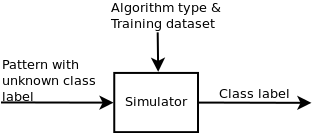
\includegraphics{fig/schema.png}
    \end{center}
    \caption{General schema of simulation environment. Input/output of the
    system}
    \label{fig:input_output}
\end{figure}

\subsection{Scope of this project} 
This paper comprises of two parts. In the first, the review of
literature and the basic notation used in the whole thesis is presented. Section
\ref{cha:Introduction} is the source of the basic
knowledge about pattern recognition. Sections \ref{cha:Rough_set}, \ref{cha:Fuzzy_logic}
present the description of algorithms used in this thesis. Additionally, this
part shows algorithm construction steps using pseudo-code.

The second part, which is the main point of this thesis, presents experiments analysis.
Paragraph \ref{cha:ExperimentAnalysis} describes the experiment environment
setting and program written in \textit{Python} to simulate all implemented
algorithms.  Results with comments are placed in
section \ref{cha:Simulation_investugations}. General
conclusions and plans for the future work are placed in sections
\ref{cha:Summary}, \ref{cha:FutureWork}, respectively. 


\section{Pattern recognition algorithms}
\label{cha:Introduction}
\subsection{Introduction}
This section is devoted for presenting information about pattern recognition
algorithms. The main purpose is to describe algorithms that are used in this
thesis. 

Pattern recognition is a wide area of science in which we are interested in
assigning label from a given set of classes to every unknown pattern. The whole 
process of classification can be divided into few phases, where each has a
significant impact on the final classification accuracy:
\begin{enumerate}
    \item Data collection
    \item Feature selection
    \item Model selection
    \item Classifier selection
    \item Training 
    \item Testing
\end{enumerate}
At first in this section few basic information and categories will be given 
about pattern recognition. Generally, the whole process of classification
can be broken down into two main categories:
\begin{itemize}
    \item supervised - incoming to the system objects are not previously
        labeled and this is the system task to find an appropriate structure of
        the data, to establish the organization of the classes basing only on
        the available data, there is no statistical or expert knowledge at a
        hand.
    \item unsupervised - in this approach incoming patterns have labels and can
        be treated as a training set. This allows the classifier can retrieve
        information from data 
\end{itemize}
In this thesis supervised learning is reconsidered because available datasets 
are labeled with class number. Further division is connected with syntactic and statistical 
approach. In former, each pattern is represented in terms of 
$d$ features (measurements) and is viewed as a point in
$d$-dimensional feature space, while the latter
is based on the characterization of the inherent structure of the 
qualitative features. For that  reason, the complex patterns can be
decomposed using a hierarchical structure in simple  sub-patterns.
The patterns are viewed as sentences belonging to a language, primitives
represents the alphabet of the language and the sentences are generated
according to a grammar which is inferred from the available training data.
EKG waveforms, textured images and shape analysis of contours are the examples
of syntactic approach.

\subsection{Problem statement for pattern recognition task}
\label{cha:Problem_statement}
In this section the problem statement will be presented in case of pattern
recognition algorithm. For the purpose of this thesis we assume a supervised learning and
denote each pattern by the label $j \in M$, where $M$ is an $m$-element set of
possible states numbered with the successive natural numbers. The state $j$ is
unknown and does not undergo the direct investigation. What can only be
measured are attributes or features by which a state manifests itself. For this
reason each object(pattern) will be described by a $d$-dimensional measured feature vector $x \in
X$. In order to classify unknown pattern algorthm uses knowledge stored in the training
set consisting of $N$ training patterns:
\begin{equation}
    S = (x_1, j_1), (x_2, j_2), \ldots, (x_N, j_N)
    \label{eq:training_pattern}
\end{equation}
In practice the decision algorithm  with learning phase should use knowledge included in the
training set $S$ and as the consequence the algorithm with learning is of the
following form:
\begin{equation}
    i=\Psi(S, x), \, i \in M
    \label{eq:decision_algorithm}
\end{equation}
In decision theory, to ensure that $\Psi$ approximates the problem as closely
as possible an additional loss function is introduced that assigns a specific
value to the loss resulting from producing an incorrect label. The particular loss
function depends on the type of label being predicted. In case of
classification problem it is zero-one loss function. This corresponds simply to
assigning a loss value of 1 to any incorrect labeling and is equivalent to computing
the accuracy of classification procedure over the set of training data.

\subsection{Rough sets}
\label{cha:Rough_set}
\subsubsection{Introduction}
\label{cha:Rough_set_introduction}
Rough sets theory represents the mathematical approach to deal with imperfect knowledge. 
In the standard standard pattern recognition task we need precise information about pattern to recognize, 
while rough sets can deal with vague or incomplete data. The problem of imperfect 
information has been tackled for a long time and it has become a crucial issue for many scientist.
One of the most prominent approaches in the recent years are fuzzy logic and rough sets.
In this section the latter approach is presented in greater details. 

Comparing with other methods, rough sets have many advantages, but one of the most important
one is its ability to works only on the raw data, with no additional information such 
as density probability in Bayesian algorithm \cite{bib38}, \cite{bib14}. The main facts about rough sets
algorithm can be summarized in few point presented below:
\begin{enumerate}
    \item simplifies data by the granulation pre-processing
    \item is able to reduce attributes
    \item generates set of easy to understand and readable decision
        \textit{IF-THEN} rules
    \item evaluates significance of data 
\end{enumerate}

When talking about rough set theory one has to understand the concept of a set 
and how a rough set is related to the classical set represented in mathematic.
From the mathematical point of view the crisp (precise) set is a collection of 
objects of interest and is uniquely determined by its elements. In other words,
it means that every element must be uniquely classified as belonging to the set 
or not (true or false). For example, the set of odd numbers is crisp because every
number is either odd or even and cannot be partially in both. 

Generally, we come across problem form the nature that are much more
complicated than simple decision whether an objects belong to the set or not. 
For some sets we cannot precisely describe element
membership. Reconsider the group of people and division into set of small and
high people. The height is not a precise but a vague concept and data vagueness can 
be met in many problems found in the nature. Here is the spot for rough sets
theory where vagueness is expressed by a boundary region of a set. 

\subsubsection{Basic notation}
\label{cha:Rough_set_basic_notation}
In rough sets theory to represent datasets (information) we introduce a notion 
called an \textit{information system} \cite{bib37}, \cite{bib39}. 
It can be described by 4-tuple
\begin{equation}
    IS = <U, Q, V, f >
    \label{eq:information_system}
\end{equation}
where the notation used in eq. (\ref{eq:information_system}) is as follows:
\begin{itemize}
    \item $U$ is the universe of discourse  which is a finite set of objects
        (patterns)
    \item $Q$ is a finite set of attribute by  which each patterns manifests
        itself (is described)
    \item $V = \bigcup V_q$, $V_q$ represents a domain of attribute $q$
    \item $f:U \times Q \rightarrow V$ is a total information function, such that
        $\bigvee_{q\in Q, x \in U} f(x,q) \in U$
\end{itemize} 
The information system can be represented as a finite table in which 
columns are labeled by attributes and each rows stands for an object from
$IS$. Over the information table we can define decision table
$T$ where the set of attributes $Q$ is disjoined into two
subset $C$ and $D$. The set $C$ is a subset of 
condition attributes, and the set $D$ contains decision attributes 
by which we can partition set $U$ into decision classes.

From the granular nature of rough sets it may happen that some objects 
in the $U$ are indistinguishable due to the limited information caused by
granulation process. Taking this into account let define an indiscernibility
relation $R \rightarrow U \times U$, representing the 
lack of knowledge about patterns in the set $U$. The indiscernibility relation on
$U$ can be extended and associated with every non-empty subset of attributes $P \subseteq Q$
and is defined by eq. (\ref{eq:indiscernibility})
\begin{equation}
    I_P = \{ (x, y) \in U \times U: f(x, q) = f(y,q), \bigvee_{q \in P}\}
    \label{eq:indiscernibility}
\end{equation}
Now having $I_P$ we can say that objects $x$ and
$y$ are $P$-indiscernible by a set of attributes $P$ if $y \, I_P \, x$. Relation
$I_P$ divides the set $U$ into blocks (concepts) of $P$-indiscernible objects.
The $P$-elementary set containing objects $P$-indiscernible with $x \in U$ is
referred as $I_P(x)$ and defined as follows:
\begin{equation}
    I_P = \left\{ y \in U: y \, I_P \, x \right\}
    \label{eq:p_indiscernible}
\end{equation}

By representing a target concept $X$ as a subset of $U$ we would like to
describe it with respect to $R$. Additionally let assume $P$ as non-empty
subset of attributes from $Q$. In rough sets reasoning an object membership to a
set can be represented in two ways:
\begin{enumerate}
    \item An object $x \in U$ certainly belongs to $X$ if
        all objects from the $P$-elementary set defined by $I_P(x)$ also belong to $X$.
        A set of all objects certainly belonging to $X$ creates the $P$-lower
        approximation of $X$ and can be represented as follows:
        \begin{equation}
            \underline{I_P} = \{ x \in U: I_P(x) \subseteq X\}
            \label{eq:lower_approximation}
        \end{equation}
    \item An object $x \in U$ can possibly belong to $X$ if at least one object
        from $P$-elementary set $I_P(x)$ can possibly belong to $X$. All the
        objects that could possibly belong to $X$ are denoted as $P$-upper
        approximation of $X$, defined as:
        \begin{equation}
            \overline{I_P} = \{x\in U: I_P(x) \, \cap \, X \neq \emptyset \}
            \label{eq:upper_approximation}
        \end{equation}
        Therefore the set $U - \overline{I_P}$ represents the negative region
        containing the set of objects that can be definitely ruled out as
        members of the target set $X$.
\end{enumerate}

The tuple $<\underline{I_P}, \overline{I_P}>$ representing a lower boundary of
the target $X$ and the upper boundary of the target $X$ creates a rough set \cite{bib34}.
Using above notion we can define $P$-boundary region which is a difference
between upper and lower approximation \cite{bib14}. 
\begin{equation}
    BN_P(X) = \overline{I_P} - \underline{I_P}
    \label{eq:boundary_region}
\end{equation}
The $BN_P(X)$ is a set of elements which cannot be certainly classified neither
as $X$ nor as not-$X$ with respect to the set of attributes $P$. If the
boundary region of $X$ is empty then the set represented by tuple
$<\underline{I_P}, \overline{I_P}>$ 
is crisp, otherwise we deal with inexact set which is called rough set. 
Until this moment we can see that rough sets concept can be defined quite generally by means of topological
operations: interior and closure, called approximations. They express the
knowledge about pattern in terms of granules, not by a precise measure
\cite{bib40}.

The illustrative example of rough sets reasoning is presented in fig. \ref{fig:rough_set_example}
\begin{figure}[H] 
    \begin{center}
        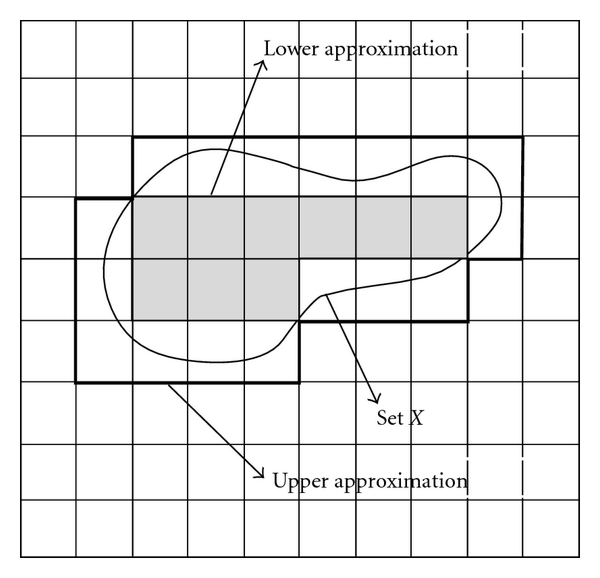
\includegraphics{fig/rough_set.png}
    \end{center}
    \caption{Rough sets example presenting lower and upper approximations}
    \label{fig:rough_set_example}
\end{figure}

\subsubsection{Rough sets indicators}
\label{cha:Rough_sets_indicators}
In rough sets theory we can define few indicators. First of all with every 
subset of $X \subseteq U$ described by $P$ subset of attributes we can 
associate an indicator called an accuracy of approximation defined as:
\begin{equation}
    \alpha_P(X)=\frac{\underline{I_P}(X)}{\overline{I_P}(X)}
    \label{eq:accuracy_approximation}
\end{equation}
The grater $\alpha_P(X)$ is, the better approximation we have which means that
many objects can be certainly classified as belonging to the target set $X$.

Another important indicator is a quality of approximation of $X \subseteq U$ by
attributes from subset $P$. It represents the percentage of correctly classified 
objects using attributes $P$ from subset $X$:
\begin{equation}
    \gamma_P(X) = \frac{\overline{I_P}(X)}{|X|}
    \label{eq:quality_approximation}
\end{equation}
Assuming that we can partition $U$ into $n$ decision classes using $P$
non-empty subset of attributes from $C$, the quality of classification can be
defined as the ration of all correctly classified objects into classes:
\begin{equation}
    \gamma_P(CLASS) = \frac{\sum_{i=1}^{n}\overline{I_P}(CL_i)}{|U|}
    \label{eq:class_quality}
\end{equation}

These indicators can be used in determining the quality of rough set algorithm
or for finding the optimal reduct. Generally, the main goal in constructing
rough sets algorithm is to obtain rule set with possible the greatest number of
certain decisions.

\subsubsection{Properties of rough sets}
The same as classical sets, rough sets can be described by the
following properties:
\begin{enumerate}
    \item $\overline{I_P} \subseteq \, X \, \subseteq \, \underline{I_P}$
    \item $\overline{I_P}(\emptyset) = \underline{I_P}(\emptyset) = \emptyset;
        \;
        \overline{I_P}(U) = \underline{I_P}(U) = U $
    \item $\overline{I_P}(X \cup Y) = \overline{I_P}(X) \cup \overline{I_P}(Y)$
    \item $\underline{I_P}(X \cap Y) = \underline{I_P}(X) \cap \underline{I_P}(Y)$
    \item $\overline{I_P}(U-X) = -\underline{I_P}(X)$
    \item $\underline{I_P}(U-X) = -\overline{I_P}(X)$
\end{enumerate}
It is easily seen that the lower and the upper 
approximations of a set are interior and 
closure operations in a topology generated by the 
indiscernibility relation $I_P(X)$. Additionally, in rough sets theory 
we can define four types of data vagueness \cite{bib40}:
\begin{itemize}
    \item $\overline{I_P}(X) \neq \emptyset,\, \underline{I_P}(X) \neq
        \emptyset$ $IF\; X$ is roughly $I_P$-definable. It means that for some
        elements from $U$ we can decide whether they belong to $X$ or $U-X$
        using $I_P$
    \item $\overline{I_P}(X) \neq \emptyset,\, \underline{I_P}(X) \neq U$ $IF\;
        X$ is internally $I_P$-indefinable. It means that we are able to decide
        which elements from $U$ belong to $U-X$, but we don't know if they
        belong to $X$ using $I_P$
    \item $\overline{I_P}(X) \neq \emptyset,\, \overline{I_P}(X) = U$ $IF\;
        X$ is externally $I_P$-definable. It means that we are able to decide
        which elements from $U$ belong to $X$, but we don't know if they belong
        to $U-X$ using $I_P$
    \item $\overline{I_P}(X) \neq \emptyset,\, \overline{I_P}(X) = U$ $IF\;
        X$ is totally $I_P$-indefinable. It means that we are unable to decide
        for any element from $U$ if it belongs to $X$ or $-X$ using $I_P$
\end{itemize}
\subsubsection{Rough sets reasoning from data}
The category description can be done in two ways:
\begin{enumerate}
    \item extensional
    \item intentional
\end{enumerate}
Each of these approaches differs in the way how pattern from dataset is
represented. To represent a concept we have to be able to identify all objects belonging 
to this category. With the former approach we have no insight 
into decision engine so we do not know how to assign new objects to the category.
In the latter approach we represent the category based on the set of rules. The same 
approach is done in rough sets algorithm where an elementary 
granules (concepts) of knowledge build blocks consisting 
of indiscernible pattern from the universe of discourse $U$. 
As stated in section \ref{cha:Rough_set_basic_notation} reconsidered dataset or
problem can be represented as a table. When decision attributes from $D$ are
added to the table it is transformed into decision table $T$ where each
row is associated with decision rule.

In this section a practical example will be presented to clear all the things
out. As an example let reconsider well-known problem of patients suffering from
flu \cite{bib39}, \cite{bib40}. The task is to decide if a patient described by 3 attributes is ill or not. Table \ref{tab:example_rough_set} 
represents an information system $IS$ about healthy patient and those suffering
from flu. Attributes: \textit{Headache}, \textit{Muscle-pain},
\textit{Temperature} are called condition attributes and denoted as ($c_i,i \in (1, \ldots, q)$),
while the attribute \textit{Flu} (last column in table \ref{tab:example_rough_set}) is considered as
a decision attribute $c_d$.
\begin{table}[H] 
    \centering
    \caption{Example dataset showing healthy patients and suffering from flu}
    \begin{tabular}{|c|c|c|c|c|c|}
        \hline 
    Patient & Headache $c_1$& Muscle pain $c_2$& Temperature $c_3$& Flu $c_d$\\ \hline \hline
    p1 & no & yes & high & yes \\ \hline
    p2 & yes & no & high & yes \\ \hline
    p3 & yes & yes & very high & yes \\ \hline
    p4 & no & yes & normal & no \\ \hline
    p5 & yes & no & high & no \\ \hline
    p6 & no & yes & very high & yes \\ \hline    
    \end{tabular}
    \label{tab:example_rough_set}
\end{table}
Each row of a decision table determines a decision rule. 


\begin{tabular}[H]{l}
    Rule 1:  IF $c_1$ IS 'NO' AND $c_2$ IS 'YES' AND $c_3$ IS 'HIGH' THEN $c_d$
    IS 'YES' \\
    Rule 2:  IF $c_1$ IS 'YES' AND $c_2$ IS 'NO' AND $c_3$ IS 'HIGH' THEN $c_d$
    IS 'YES' \\
    Rule 3:  IF $c_1$ IS 'YES' AND $c_2$ IS 'YES' AND $c_3$ IS 'VERY HIGH' THEN
    $c_d$ IS 'YES' \\
    Rule 4:  IF $c_1$ IS 'NO' AND $c_2$ IS 'YES' AND $c_3$ IS 'NORMAL' THEN
    $c_d$ IS 'NO' \\
    Rule 5:  IF $c_1$ IS 'YES' AND $c_2$ IS 'NO' AND $c_3$ IS 'HIGH' THEN $c_d$
    IS 'NO' \\
    Rule 6:  IF $c_1$ IS 'NO' AND $c_2$ YES 'NO' AND $c_3$ IS 'VERY HIGH' THEN
    $c_d$ IS 'YES'  
\end{tabular}


After analyzing table \ref{tab:example_rough_set} it is noticeable that some
patients cannot be distinguished between each other, for example $p2$ and $p5$.
It is possible to generate different indiscernible relations based on 
the chosen attributes. In case of \textit{Headache} attribute patients: $p2$,
$p3$, $p5$ are indiscernible; patients $p2$, $p5$ are
indiscernible with respect to attributes \textit{Headache},
\textit{Muscle-pain} and \textit{Temperature}, or if we use \textit{Headache}
and \textit{Muscle-Pain} the set $U$ can be divided into three sets:
\{$p1$, $p4$, $p6$\}, \{$p2$, $p5$\}, \{$p3$\}.

Now it is time for defining key features of rough sets. Over the table
\ref{tab:example_rough_set} we can define two concepts (target sets):
\textit{Flu} and \textit{Not Flu}. For the first concept the lower approximation
set of patient certainly having flu is \{$p1$, $p3$, $p6$\}, while the upper
approximation of patients possibly suffering from flu is \{$p1$, $p2$, $p3$,
$p5$, $p6$\}. The boundary region for concept \textit{Flu} is a set of \{$p2$, $p5$\} 
patients. For the concept \textit{Not Flu} the lower approximation is the set
\{$p4$\}, whereas the upper approximation is the set \{$p2$, $p4$, $p5$\}. Again the 
boundary region is the set \{$p2$, $p5$\}.

Additionally, we can measure the accuracy of approximation $\alpha_P(x)$ for each concept.
This can indicate if the set of attributes used for describing the concept is correctly
chosen. For the \textit{Flu} concept where $X$=\{$p1$, $p2$, $p3$, $p6$\} is described by
set of attributes $P$=\{\textit{Headache}, \textit{Muscle-pain},
\textit{Temperature}\} the accuracy of approximation is:
$$\alpha_P(Flu) = \frac{3}{5}$$
On the other hand when we take only one attribute $P$=\{\textit{Temperature}\}, then we get lower approximation of 
\{$p3$, $p6$\} and upper approximation of \{$p1$, $p2$, $p3$, $p5$, $p6$ \}
resulting in:
$$\alpha_P(Flu) = \frac{2}{5}$$
To sum up, $\alpha_P(x)$ is a very important indicator in
rough sets theory and tells which attributes better characterize target
concept. This example has shown that because of the granule representation of
knowledge in rough sets approach some object cannot be discerned. It is very
important to choose proper condition attributes because this determines how
upper and lower approximations are represented by objects from $U$. 


\subsection{Fuzzy logic}
\label{cha:Fuzzy_logic}
\subsubsection{Introduction}
In fuzzy logic an element membership to a set is described by a membership function 
which assigns value from interval $[0, 1]$:
\begin{equation}
    \mu_A:U\rightarrow [0,1], \, A \subseteq U
    \label{eq:fuzzy_function}
\end{equation}
The properties of membership function $\mu$ are as follows:
\begin{itemize}
    \item $\mu_{\emptyset}(x) = 0, \, x \in U$
    \item  $\mu_{U}(x) = 1, \, x \in U$
    \item  $\mu_{X}(x) \leq \mu_{Y}(x), \, IF X \subseteq Y$
    \item  $\mu_{\overline{A}}(x) = 1 - \mu_{A}(x), \, x \in U$
\end{itemize}
where $\emptyset$ is an empty set and $\overline{A}$ is the complement of the
set $A$.

Fuzzy logic is a superset of Boolean logic that 
has been extended to handle the concept of partial truth - values between ``completely 
true'' and ``completely false'' \cite{bib6}, \cite{bib12}. This theory was introduced by 
Dr. Lotfi Zadeh in the 1960's as a tool for modelling the uncertainty of natural language. 
This approach can be applied to many problems, analyze only few examples:
\begin{itemize}
    \item Days of a week- there is a question which day is mostly associated
        with a weekend. Generally, we would assume that the membership value
        $g$ associated with each day will be as follows:
        \{Monday=0, Tuesday=0.2, Wednesday=0.4, Thursday=0.5, Friday=0.7,
        Saturday=1.0, Sunday=0.9\}
    \item The seasons- there is not evident boundary when one season stops and
        another starts. This example can be illustrated quite precisely by fig.
        \ref{fig:seasons}.
        \begin{figure}[H]
            \begin{center}
                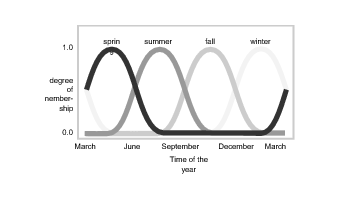
\includegraphics{fig/seasons.png}
            \end{center}
            \caption{Example of how fuzzy logic can be used to describe the
            season of the year}
            \label{fig:seasons}
        \end{figure}
    \item The height: small and tall definitions- from the group of people it
        is hard to define who is tall and who is small interchangeably. To
        solve this problem we can define the concept \textit{Tall} and assign
        value to each person describing its value. This process is presented in
        fig. \ref{fig:fuzzy_tall}
        \begin{figure}[H]
            \begin{center}
                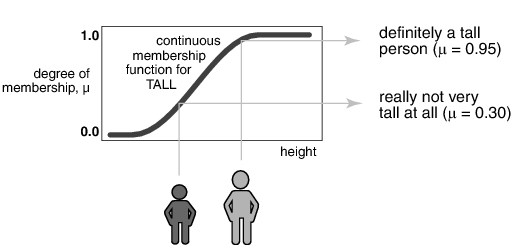
\includegraphics{fig/fuzzy_tall.png}
            \end{center}
            \caption{Fuzzy approach for defining person height}
            \label{fig:fuzzy_tall}
        \end{figure}
\end{itemize}

As in the section \ref{cha:Rough_set_introduction}, let reconsider the problem of defining 
if person is small or tall more deeply. First of all, we have to define a fuzzy
set (concept) \textit{Tall} which will answer the question 
"to what degree is person x tall?". Zadeh describes \textit{Tall} as a
linguistic variable, which represents our cognitive category of "tallness"
\cite{bib25}. To each person in the universe of discourse, 
we have to assign a degree of membership in the fuzzy subset \textit{Tall}
based on the membership function (for example the same as presented in fig.
\ref{fig:fuzzy_tall}). Table \ref{tab:fuzzy_logic_example} shows an example of fuzzy
reasoning:
\begin{table}[H]
    \centering
    \caption{Table describing how person is tall by the fuzzy logic linguistic
    variable}
    \begin{tabular}{|c|c|c|}
        \hline
        Person & Height [m] & degree of tallness \\ \hline \hline
        p1 & 1.5 & 0.0 \\ \hline
        p2 & 1.6 & 0.2 \\ \hline
        p3 & 1.7 & 0.4 \\ \hline
        p4 & 1.8 & 0.5 \\ \hline
        p5 & 1.9 & 0.6 \\ \hline
        p6 & 2.0 & 1.0 \\ \hline
    \end{tabular}
    \label{tab:fuzzy_logic_example}
\end{table}

Fuzzy numbers are fuzzy subsets generated over the attribute domain. 
They have a peak or plateau with membership grade 1, over which the 
members of the universe are completely in the set.  The membership 
function is increasing towards the peak and decreasing away from it. 
There are different types of membership functions and their usage 
strongly depends on the type of reconsidered problem. One of the most 
commonly used in the literature are: triangular, trapezoidal, Gaussian shapes
(see example in fig. \ref{fig:fuzzy_example_1}).

\subsubsection{Fuzzy reasoning from data}
Reasoning in fuzzy logic is based on decision rules the same as in rough sets
approach \cite{bib11}. 
Rules are expressed in the form of IF \textit{COND} THEN \textit{DECISION} 
which can be divided into antecedent set ($A_{ri}, \, i \in (1, \ldots, q)$) and one consequent determining the
output of the rule. In the pattern recognition task when we deal with patterns
described by $d$ features rules have the form presented by eq. (\ref{eq:rule_example})
\begin{equation}
    IF\, x_1=A_{r1}\, AND\, x_2=A_{r2}\, AND\, \ldots\, AND\, x_d=A_{rd}\, THEN\,
class\, C_r\, with \, CF_r
    \label{eq:rule_example}
\end{equation}

The \textit{AND}, \textit{OR}, and \textit{NOT} operators of 
Boolean logic exist in fuzzy logic and are usually defined as the minimum, maximum,
and complement. When they are defined this way, they are called the Zadeh
operators \cite{bib2}.

Fuzzy logic classification is based on three main steps:
\begin{enumerate}
    \item Fuzzyfication- in the fuzzyfication process we 
        convert continuous quantity into fuzzy number based on the appropriate
        membership function value. It requires defining
        membership grade of crisp input $x$ in the fuzzy set.
    \item Rule induction- there are different types of fuzzy inference systems,
        but one of the most commonly used (the same as in this paper) is
        Mamdani inference system \cite{bib46}.
    \item Deffuzification- the process of producing a quantifiable result in
        fuzzy logic from given fuzzy sets and corresponding membership degrees. 
\end{enumerate}
The whole process of fuzzy reasoning is presented in fig.
\ref{fig:fuzzy_reasoning}
\begin{figure}[H]
    \begin{center}
        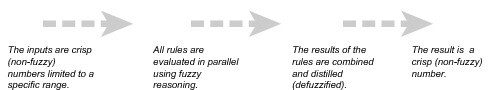
\includegraphics[width=\textwidth]{fig/fuzzy_steps.png}
    \end{center}
    \caption{Steps applied in fuzzy reasoning.}
    \label{fig:fuzzy_reasoning}
\end{figure}

Let reconsider a simple example, which should clear all ambiguities (the following 
example is based on \cite{bib0}). The problem is connected with estimating the
level of risk involved in software engineering project. There are two input
to the system (funding, staffing) and one output
(risk). Membership functions are represented as triangular shapes (fig. \ref{fig:fuzzy_example_1}) 
\begin{figure}[H]
    \begin{center}
        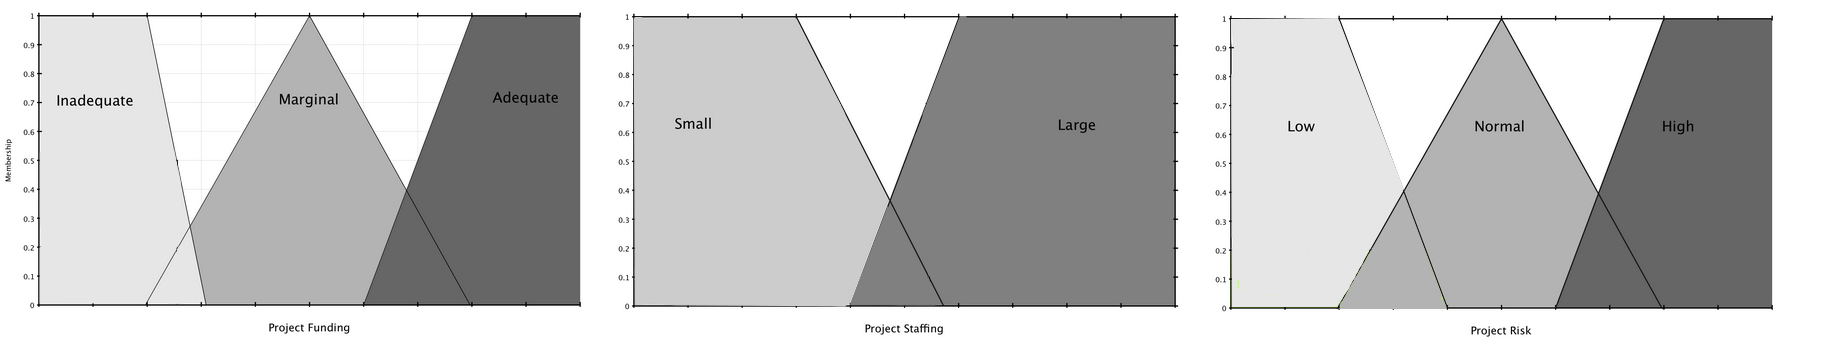
\includegraphics[width=\textwidth]{fig/fuzzy_example_1.png}
    \end{center}
    \caption{Input and output fuzzy linguistic variables for the described
    system.}
    \label{fig:fuzzy_example_1}
\end{figure}
The next important thing in fuzzy logic beside fuzzy values are fuzzy rules. In
this problem they are provide a priori and are in the following way:
\begin{table}[H]
    Rule 1: IF funding IS adequate OR funding IS small THEN risk IS
    low \\
    Rule 2: IF funding IS marginal AND staffing IS large THEN risk IS
    normal \\
    Rule 3: IF funding IS inadequate THEN risk IS high
\end{table}
Let say that we want to calculate project risk for inputs: funding~$=35$ and
staffing~$=60$. 
\begin{enumerate}
    \item The first step is to convert crisp values into fuzzy representation.
        Activating each input membership functions fuzzy values are as follows:
        $$
            \begin{array}[H]{l}
                input \;1 \\ \hline
                \mu_{inadequate}(35) = 0.5 \\
                \mu_{marginal}(35) = 0.2 \\
                \mu_{adequate}(35) = 0.0 \\ \\
                input 2 \\ \hline
                \mu_{small}(60) = 0.1 \\
                \mu_{large}(60) = 0.7 \\ 
            \end{array}
        $$
    \item Now it is time f or rule induction where OR is treated as a $max$ operator, AND
        as $min$ operator. 
        $$
            \begin{array}[H]{ll}
                Rule \,1: & \mu_{low} = 0.0 + 0.1 = 0.1 \\
                Rule \,2: & \mu_{normal} = 0.2\cdot 0.7 = 0.14 \\
                Rule \,3: & \mu_{high} = 0.5 \\
            \end{array}
        $$
    \item After performing clipping of consequent membership functions for each
        rule (example given in fig. \ref{fig:fuzzy_centroid}), the final crisp output can be calculated. It is done by
        defuzzification method, where one of the most commonly used is a centroid
        formula given by eq. (\ref{eq:fuzzy_centroid}) \cite{bib0}, \cite{bib1}.
        \begin{equation}
            CO = \frac{\sum\nolimits_{x=a}^{b}\mu_A(\chi)\cdot
            x}{\sum\nolimit_{x=a}^{b}\mu_A(\chi)}
            \label{eq:fuzzy_centroid}
        \end{equation}
        \begin{figure}[H]
            \begin{center}
                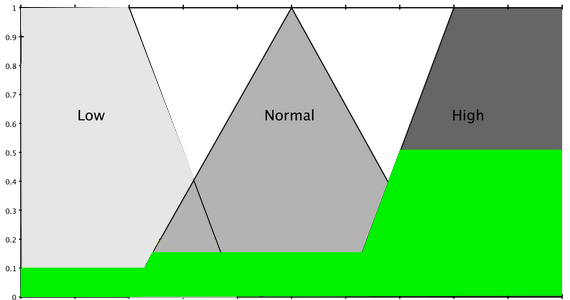
\includegraphics[width=0.6\textwidth, height=0.4\textwidth]{fig/fuzzy_centroid.png}
            \end{center}
            \caption{Example of clipping the consequent membership function
            as the result of rule induction}
            \label{fig:fuzzy_centroid}
        \end{figure}
        Using eq. (\ref{eq:fuzzy_centroid}) the output of the system is as follows:
        $$
        CO = \frac{(0+10+20)\cdot 0.1 + (30+40+50+60)\cdot 0.14 + (70 + 80 + 90
        + 100)\cdot 0.5}{0.1\cdot 3 + 0.14\cdot 4 + 0.5\cdot 4 } = 69.3
        $$
    It means that for input values funding~$=35$ and staffing~$=60$ the project
    risk is about $69\%$.
\end{enumerate}
\subsubsection{Genetic-based machine learning approaches}
In the literature one can find many examples of fuzzy logic applications
\cite{bib3}, \cite{bib9}.
Generally, there are two main approaches:
\begin{enumerate}
    \item some expert knowledge is available and fuzzy rules are created
        beforehand.
    \item no knowledge about data set is present so some techniques of data
        mining must be applied to extract rules from the training set.
\end{enumerate}
At this point it must be strongly emphasized that in this thesis the main focus is based on
fuzzy algorithm for pattern recognition task where there is no prior knowledge 
about fuzzy system and decision rules. There are different approaches for
construction fuzzy logic algorithm from raw dataset, for example optimization techniques
such as gradient descent or heuristic algorithms \cite{bib8}, \cite{bib16},
\cite{bib28}. In this paper the genetic algorithm
is proposed for creating an optimal rule set. 

One can wonder what is the purpose of applying genetic algorithm into rule
generation. For the simplicity let reconsider such a case. $N$ training
patterns are available and nothing more. Now the following question arises: 
how to properly divide the feature space into fuzzy set, and how to generate
decision rules when there is no expert knowledge. The simplest and
straightforward solution is to create let say 10 triangular membership functions for each
attribute, and check each possible combination. Is this approach optimal? The
efficiency of this solution strongly depends on the complexity of the problem.
For $d$-dimensional feature space and $k$ fuzzy membership function per each attribute
the number of possible combination for generating one rule is equal to $k^d$.
For greater $d$ (for example wine dataset from \textit{UCI} repository has 13
attributes) it is impossible to find the proper combination in a reasonable
time. Here is an open spot for genetic algorithm to show its searching
abilities.

There are two main methods of genetic-based machine learning approaches
\cite{bib30}, \cite{bib31}:
\begin{enumerate}
    \item Michigan template- it is a population of fuzzy rules and a single
        fuzzy rule is handled as an individual (see fig. \ref{fig:michigan}). 
        The evaluation of each fuzzy rule is performed by classifying all the 
        given training patterns by the available rule set $N_{rule}$. At the 
        end of each iteration new individuals are created through genetic operators 
        and merged to the current population. For the next generation $N_{rule}$ 
        best individuals are taken. The whole procedure can be summarized as follows:
        \begin{enumerate}
            \item Generate $N_{rule}$ fuzzy rules
            \item Evaluate the fitness of each fuzzy rule in the current
                population
            \item Generate $N_{replace}$ fuzzy rules using genetic operators
            \item Merge $N_{replace}$ fuzzy rules with current population and
                choose the best $N_{rule}$ individuals for the next generation
            \item Return to point $(b)$ is stopping condition is not fulfilled
                (number of generations)
        \end{enumerate}
        \begin{figure}[H]
            \begin{center}
                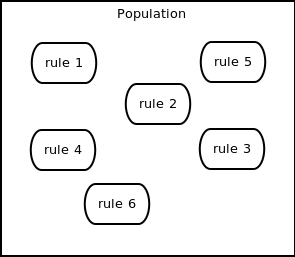
\includegraphics[width=0.5\textwidth, height=0.4\textwidth]{fig/michigan.png}
            \end{center}
            \caption{Example of Michigan approach for constructing Genetic
            Fuzzy logic algorithm}
            \label{fig:michigan}
        \end{figure}
    \item Pittsburgh template- in this approach a set of fuzzy rules is handled
        as an individual (see fig. \ref{fig:p}). In this case the length of a single individual is
        equal to $n\cdot N_{rule}$, where $n$ is the length of single fuzzy rule.
        Algorithm starts with $N_{pop}$ randomly generated rule sets. The
        fitness value of a single individual is the number of correctly
        classified patterns in the training set by a given rule set.
        The procedure for algorithm is as follows:
        \begin{enumerate}
            \item Generate $N_{pop}$ individuals consisting of $N_{rule}$ fuzzy
                rules each
            \item Calculate the fitness value of each rule set (individual)
            \item Generate $N_{replace}$ new rule set using genetic operators.  
            \item Merge $N_{replace}$ fuzzy rule sets  with current population and
                choose the best $N_{pop}$ individuals for the next generation
            \item Return to point $(b)$ is stopping condition is not fulfilled
                (number of generations)
        \end{enumerate}
        \begin{figure}[H]
            \begin{center}
                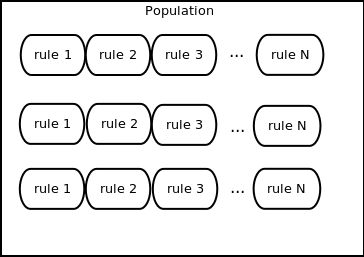
\includegraphics[width=0.5\textwidth, height=0.4\textwidth]{fig/pittsburgh.png}
            \end{center}
            \caption{Example of Pittsburgh approach for constructing Genetic
            Fuzzy logic algorithm}}
            \label{fig:p}
        \end{figure}
\end{enumerate}
In this thesis the first approach will be implemented which means that
individual is modelled as a single rule. 

\subsection{Attribute reduction}
\label{cha:Attribute_reduction}
Many problem are complex and multidimensional. For example Sonar dataset from
\textit{UCI} Repository has 60 attributes describing a single pattern. 
Usually we hope to recognize pattern in a relatively
lower dimensional to reduce cost in measuring and processing information and
enhance the interpretability of learned models. Feature selection or reduction 
is done for classifiers to remove the noise and superfluous data. Generally,
this is not an easy task and requires a lot of computation \cite{bib1}, \cite{bib5}.  

A reduct is a set of attributes that ensures the same classification of
elements from $U$ as the rudimentary set of attributes. More than one reduct
can exist for one information system. The core of attributes is the set of
attributes from $Q$ that all the attributes are indispensable. An attribute is
dispensable if the following criterion is fulfilled:
$$I(P) = I(P-{a}), \, \textrm{for} \, \{a\} \in P \subseteq  Q $$

In the literature there are many examples of how to apply attribute reduction
\begin{itemize}
    \item information measures
    \item distance measures
    \item dependence measures
    \item consistency measures
\end{itemize}
Different approaches provide various results and their application strictly
depend on the type of data. One of the best known methods are Principal
Component Analysis, Factor analysis or optimization and heuristic techniques.
In the recent years heuristic techniques are very often used because of their
speed and searching abilities. A lot of work has been devoted for feature
extraction and this is not the intention to explore this area of research.
Basing on the results conclusions presented in the literature, in this thesis a 
genetic algorithm is proposed for extracting valuable features from the set of 
all attributes \cite{bib27}, \cite{bib48}.

\subsection{Genetic algorithm}
\label{cha:Genetic_algorithm}
Genetic Algorithm is an element of evolutionary computation, which is a 
rapidly growing area of soft computing \cite{bib42}, \cite{bib43}. GA is based on the principles of
natural selection and genetic modification. As optimization methods, GA 
operates on a population of points, designated as individuals. Each 
individual of the population represents a possible solution of the 
optimization problem. Individuals are evaluated depending upon their 
fitness which indicates how well an individual of the population solves 
the optimization problem. To sum up, GA has the following general features:
\begin{enumerate}
    \item GA operates with a population of possible solutions (individuals) 
        instead of a single individual. Thus, the searching process can be 
        carried out in a parallel form or sequentially.
    \item GA is able to find the optimal or sub-optimal solutions in complex
        and large search spaces. Moreover, it can be applied to nonlinear 
        optimization problems with constraints defined in discrete or continuous 
        search spaces.
    \item GA examines many possible solutions at the same time, so there is a 
        higher probability that the search process can converge to an optimal solution.
\end{enumerate}
There are four main parts in each GA process to reconsider (graphically
presented as a flow chart \ref{fig:genetic_scheme}):
\begin{enumerate}
    \item the problem representation or encoding
    \item fitness or objective function definition
    \item fitness-based selection
    \item evolutionary reproduction of candidate solutions (individuals or chromosomes). 
\end{enumerate}
\begin{figure}[H]
    \begin{center}
        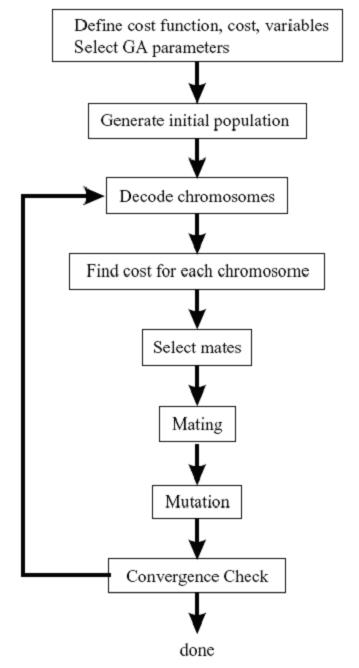
\includegraphics[height=0.5\textwidth]{fig/genetic.png}
    \end{center}
    \caption{Diagram representing phases in genetic algorithm evaluation}
    \label{fig:genetic_scheme}
\end{figure}

Genetic algorithms are widely used as a search techniques in the various fields. 
In this thesis it will be used for finding an optimal cuts in the attribute space and to 
apply attribute reduction. The success of a genetic algorithm can be quantified by estimating 
the cost, time required and the quality of final obtained solution. 

In the literature there can be found many examples of how GA is useful in solving hard 
optimizations problems, but beside unquestionable advantages there also exist downsides. 
A traditional GA without any diversity maintenance mechanism often suffers from getting 
stuck on the suboptimal peaks, because almost the entire GA population would have converged 
to a single peak, as a result of the rapid loss of population diversity \cite{bib44}, \cite{bib45}. 

There is a great deal of work showing how to set the optimal parameters in an evolutionary 
algorithm to obtain required speedup and solution accuracy, but this is not the main issue 
in this thesis. For more exact information see \cite{bib42}, \cite{bib43}.

When designing genetic algorithm one of the most important things to ensure proper crossover 
and mutation operations. More precise information about these operators will be
presented in section \ref{cha:Algorithm_construction}.

\subsection{Hybrid classifiers} 
\label{cha:Hybrid_classifiers}
In the recent years, there is an increasing interest in methods of combining
multiple learning systems into hybrid one \cite{bib5}, \cite{bib6}. The main advantage of such approach
is its ability to find different explanation for the dataset for each
classifier. If classifiers make errors on different parts of the feature space
it is possible that the ensemble of classifiers will complement each other and
the final classification will be better. 

Generally, there are two types of hybrid classifiers (example presented in fig.
\ref{fig:hybrid}:
\begin{enumerate}
    \item multiexpert systems- classifiers work in parallel, each of them is
        trained and tested on the same data and independent decisions are
        combined to compute the final result. The most common example is a
        majority voting.
    \item multistage systems- classifiers are connected in a sequence where the
        next classifier is trained and used for classification only if the
        previous classifier rejected the pattern. 
\end{enumerate}
It is hard to determine which approach is the best. Each system has its pros
and cons and the choice depends of the type of dataset and available
classifiers. In this thesis the second approach is implemented where the first
segment is built by rough sets classifier and the second one is constructed by
fuzzy logic.
\begin{figure}[H] 
    \begin{center}
        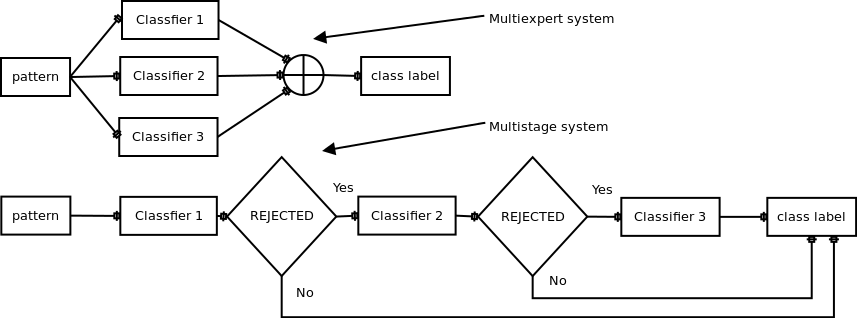
\includegraphics[width=\textwidth]{fig/hybrid.png}
    \end{center}
    \caption{Example of two approaches for constructing hybrid classifiers}
    \label{fig:hybrid}
\end{figure}


\section{Algorithm construction}
\label{cha:Algorithm_construction}
In this section basic information about algorithm construction will be
presented. For the classification task four algorithms were implemented and
compared.

At the beginning, we start with the basic algorithm of rough sets, later present rough sets
algorithm with modification of decision rules and at last the multistage hybrid 
algorithm consisting of genetic algorithm, rough sets and fuzzy logic is shown in 
greater details. 
\subsection{Rough sets algorithm construction}
\label{cha:Algorithm_construction_rough_set}
The basic rough sets algorithm with constant step of granulation
can be summarized in six steps \cite{bib34}, \cite{bib35}:
\begin{enumerate}
    \item If the attributes are the real numbers then the granulation preprocessing 
        is needed first. To calculate the proper interval eq. (\ref{eq:interval})
        is used:
        \begin{equation}
            v_{pi}^{i} = \frac{f_{i}}{G}\cdot(f_{i, max}-f_{i,min})
            \label{eq:interval}
        \end{equation}
        where $v_{pi}^{i}$ is the interval label for $i$-th attribute; $f_i$ is
        the $i$-th real attribute value for pattern $x$, $f_{i,min}$ and
        $f_{i,max}$ denote the extend of the $i$-th feature calculated in the
        training phase. If for any attribute from $x$ in the testing phase 
        $f_i > f_{i, max}$ then $v_{pi}^{i}=G-1$ or $f_i < f_{i, min}$ then
        $v_{pi}^{i}=0$, in other cases eq. (\ref{eq:interval}) is applied.

        After this step, the value of each attribute is represented 
        by the number of interval in which this attribute is included. For each
        attribute from $l=(1, \ldots , q)$ we choose the same numbers of
        intervals $K_l$ called step of granulation $G$. For the $l$-th attribute 
        denoted by $v^l_{p_l}$ it is defined its $p_l$ interval from $p_l=(1, \ldots, K_l)$
    \item Using training dataset construct the decision table $T$ where each
        row represents a pattern. Over the table $T$ define the set $FOR(C)$ of decision rules of
        the following form:
        $$IF \, (x_1 = v_{p_1}^1) \, AND \, (x_2=v_{p_2}^2) \, AND \, \ldots \,
        (x_q=v_{p_q}^q) \, THEN \, \Psi(S, x)=j$$
        Each generated rule is evaluated and the strength factor is assigned to
        it determining the accuracy of approximation (see section \ref{cha:Rough_sets_indicators})
    \item For the created set of formulas $FOR(C)$ for each $j=1, \ldots, m$
        an algorithm calculates lower $\underline{I_P}$, upper $\overline{I_P}$ approximations and the boundary
        region $BN_P$ which are determined by the set of conditional attributes $P
        \subseteq Q$
    \item In order to classify new pattern $x$ algorithm looks for matching rules in the
        set $FOR(C)$ (rule is activated if the left condition is fulfilled by
        attributes describing $x$).
    \item If there is only one matching rule $r$, then the pattern $x$ is
        classified to the class which is indicated by $r$ decision attribute $j$, 
        because for sure such a rule is belonging to the lower approximation of all rules 
        indicating $j$. Rule $r$ is denoted as a \textit{certain} rule.
    \item If there is more than one matching rule in the set $For(C)$, 
        it means that the recognized pattern should be classified by the 
        rules from the boundary regions and in this case as a decision
        algorithm takes the index of boundary region for which the strength of corresponding 
        rule is maximal. All activated rules are denoted as \textit{possible}
        rules.
    \item In other cases: no appropriate rule was found or few rules have the same strength
        factor then the unknown pattern $x$ is rejected.
\end{enumerate}
\subsection{Rough sets algorithm construction with modification of decision rules}
\label{cha:Algorithm_construction_rough_set_modification}
It can happen that for certain number of intervals algorithm cannot find patterns in
the training set, so as the consequence dummy rule are generated, useless in the
classification process (the strength of the rule is 0). 
The main drawback of algorithm presented in section \ref{cha:Algorithm_construction_rough_set}
is the fact that it starts with an arbitrary chosen step of granulation and its accuracy strongly
depends on it. In this section the recursive modification of the previous algorithm is
presented allowing for automatically changing the step of granulation is
the pattern $x$ is rejected. The modification is as follows \cite{bib36}:
\begin{enumerate}
    \item Algorithm starts with an arbitrary chosen step of granulation $G$, 
        generally it is a high value to ensure that recursion can be invoked
        by decreasing $G$. Shortly speaking, we divide every domain of feature into $G$
        intervals. At first algorithm repeats the whole procedure 1-6 described
        in the previous section.
    \item If for the pattern $x$ algorithm cannot find neither certain nor possible
        decision rule, it means that there is no proper representation in the learning set. 
        In such a situation algorithm tries to find matching rule by decreasing recursively
        the current interval $G$ by factor $\epsilon=1$ for every condition attribute $l=1, \ldots, q$
        until the proper rule is found. If \textit{certain} rule or
        \textit{possible} rules with maximum strength are induced then the algorithm
        returns decision attribute $j$, otherwise if for every attribute $G=1$, then the pattern $x$ is rejected.
\end{enumerate}
The recursion is time consuming so to enhance the process of finding the proper
decision formulas for different $G$ the decision set $FOR(C)$ are stored in the memory
for faster retrieval.

\subsection{Fuzzy logic algorithm construction}
\label{cha:Algorithm_construction_fuzzy_logic}
\subsubsection{Problem formulation}
\label{cha:Fuzzy_logic_basic_problem_formulation}
In the fuzzy logic algorithm one of the most important key is creation of rules
which will ensure proper classification. When there is no expert knowledge about
dataset it is not an easy task to generate them from scratch. In the literature
one can find many practical examples of how to generate \textit{IF-THEN} rules, from
the statistical tools to heuristic algorithms. In the recent the most appealing
and effective approach is genetic algorithm \cite{bib4}, \cite{bib13}, \cite{bib23}

For the algorithm construction we have to make few assumptions:
\begin{itemize}
    \item For the learning procedure $N$ training patterns are available
    \item A set $F$ of linguistic values and their membership functions is given
        for describing each attribute. 
\end{itemize}
The second point is the most important and the choice of the proper membership
functions affects the classification accuracy \cite{bib17}, \cite{bib6}. It requires in-depth explanation
of how set $F$ is generated in this thesis, how to partition each attribute into 
linguistic values and how to describe each membership function. Genetic
algorithm is used here for finding an optimal parameter settings. 

Fig. \ref{fig:fuzzy_example} shows an example of how to generate fuzzy set $F$ of
possible membership functions. In this example $14$ membership functions are used. 
Each function has a subscript defining its linguistic value and a proper
location in the feature space. To emphasize the complexity of the problem let take 
into account that each attribute is divided in the same way as depicted in fig. \ref{fig:fuzzy_example}. 
Having $d$-dimensional feature space, the number of all possible combinations of membership functions for
rule construction is equal to $14^d$. It is impossible to evaluate each potential solution it is
in a reasonable time \cite{bib27}, \cite{bib33}. 
\begin{figure}[H]
    \begin{center}
        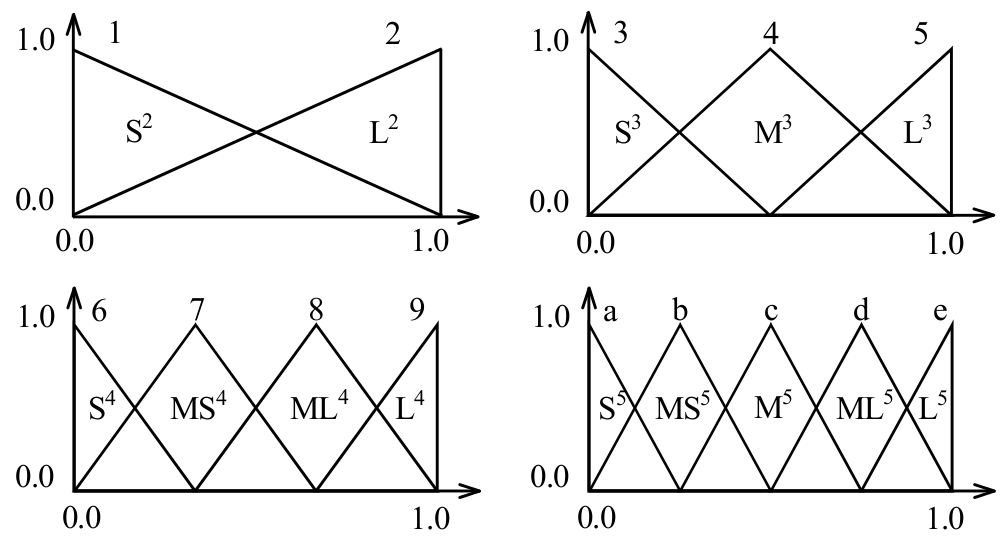
\includegraphics[width=\textwidth]{fig/fuzzy_example.png}
    \end{center}
    \caption{Example fuzzy partition set for an attribute}
    \label{fig:fuzzy_example}
\end{figure}
For classification task single fuzzy rule is in the following form
\cite{bib30}, \cite{bib20}:
$$R_r:\, IF\, x_1=A_{r1}\, AND\, x_2=A_{r2}\, AND\, \ldots\, AND\, x_d=A_{rd}\, THEN\,
class\, C_r\, with \, CF_r$$
where $x=(x_1, x_2, \ldots, x_d)$ is a $d$-dimensional pattern vector; $A_{ri}$
is an antecedent fuzzy set with a linguistic label (taking into account the
example from \ref{fig:fuzzy_example} $A_{ri}$ can have one label from the set
$\{1, 2, \ldots, 9, a, b, \ldots, e \}$); $C_r$ is a consequent fuzzy set
determining the class label $\{1, \ldots, m\}$, $CF_r$ is a rule strength; $r$
denotes the number of the rule from the set of all possible rules $\{1, \ldots, N_{rule}\}$. 
Generally, $N_{rule}$ is about ten or twenty. 
\subsubsection{Rule generation}
\label{cha:Fuzzy_logic_rule_generation}
The process of rule generation for fuzzy logic without the expert knowledge is
complex and done in couple steps. At first, using available
training set, generate randomly $N_{rule}$ rules. For
each training pattern $x_p$ calculate the compatibility grade of a single rule
connected with antecedent part $A_r = (A_{r1}, A_{r2}, \ldots, A_{rd})$ using
the product operator of each membership function $\mu_{A_{ri}}$ determined for
$A_{ri}$:
\begin{equation}
    \mu_{A_r}(x_p)=\mu_{A_r1}(x_p)\cdot\mu_{A_r2}(x_p)\cdot\ldots\mu_{A_rd}(x_p)
    \label{eq:mu_product}
\end{equation}
If we know how to calculate the compatibility grade of each training pattern
now we can determine $C_r$ and $CF_r$ for each rule. The fuzzy probability
$P(class\, j|A_r)$ of class $j$, $j=(1, \ldots, m)$ is given by eq. (\ref{eq:fuzzy_probability})
\begin{equation}
    Pr(class \, j|A_r) = \frac{\sum\limits_{x_p \in class\,
    j}\mu_{A_r}(x_p)}{\sum\limits_{p=1}^m\mu_{A_r}(x_p)}
    \label{eq:fuzzy_probability}
\end{equation}
For the $r$-th rule $R_r$ the label of class is assigned according to the
winning rule, which means that the label with maximal probability is chosen:
\begin{equation}
    R_r: C_r = max\limits_{j=\{1, \ldots, m\}}\{Pr(class\,j|A_r)\}
    \label{eq:fuzzy_max}
\end{equation}
In the learning phase it can happen that rule $R_r$ can be activated by
patterns coming from different classes. To ensure the proper classification, each
rule has a strength factor which tells how precisely rule $R_r$ predicts the
consequent class $h$.
\begin{equation}
    R_r: CF_r=Pr(class\, j|A_r) - \sum\limits_{j=1, j\neq C_r}^MPr(class\,j|A_r)
    \label{eq:fuzzy_strength}
\end{equation}
If $CF_r$ in eq. (\ref{eq:fuzzy_strength}) is negative then rule $R_r$ is
denoted as \textit{dummy} and is not taken for further reasoning, otherwise it is used in
defuzzification process to determine the final class label \cite{bib18}, \cite{bib26}.
\subsubsection{Fuzzy reasoning}
\label{cha:Fuzzy_reasoning}
Let assume that $N_{rule}$ fuzzy rules are generated with indicators $C_r$,
$CF_r$ determined by eq. (\ref{eq:fuzzy_max}), (\ref{eq:fuzzy_strength}). 
Then the process of classification is done as follows:
\begin{equation}
    \Psi(S, x_p) =  C_q \leftarrow max_{j=\{1,\ldots,
    M\}}\{\mu_{A_{q}}(x_p)\cdot CF_r\}
    \label{eq:fuzzy_classification}
\end{equation}
The label of the class for unknown pattern is determined by a winner rule $R_w$
that has the maximum compatibility grade and the rule strength $CF_r$.

If multiple fuzzy rules have the same maximum product $\mu_{A_r}$ but different
consequent classes then the classification is rejected. The same action is
taken if no fuzzy rule is compatible with the incoming pattern $x_p$.
\subsubsection{Genetic algorithm for  fuzzy algorithm construction}
\label{cha:Fuzzy_logic_genetic_algorithm}
In this section genetic algorithm will be described in greater details. This
algorithm was used to generate initial number $N_{rule}$ of fuzzy rules for
classification. 
Basic assumptions:
\begin{itemize}
    \item Fuzzy rule encoding is the same as presented in section \ref{cha:Fuzzy_logic_basic_problem_formulation}
    \item Training data set is given with $N$ patterns
    \item Triangular membership functions are used and described by 2-tuple
        $(a, b)$, where $a$ is the center value (where $\mu(x)=1$), and
        $b$ determines left and right extend of membership function, respectively.
        \begin{equation}
            \mu(x) = 
            \begin{cases}
                \frac{-1}{b}\cdot x + \frac{a+b}{b} &
                x \geq a \, and \, x \leq (a+b) \\
                \frac{1}{b}\cdot x - \frac{a-b}{b} &
                x \geq (a - b)\, and\, x < a \\
                0 & otherwise
            \end{cases}
            \label{eq:fuzzy_function}
        \end{equation}
    \item Possible partitions of the feature space are determined in the same
        way as in the example presented in fig. \ref{fig:fuzzy_example}
    \item Genetic algorithm uses standard operations such as cross-over,
        mutation, population generation, fitness evaluation.
    \item As the template for genetic fuzzy algorithm Michigan approach is
        used which means that we have $N_{rule}$ number of individuals in the
        population
\end{itemize}
Next few step will present the whole structure of genetic algorithm used in
this section:
\begin{itemize}
    \item Chromosome representation and encoding: 
        \begin{itemize}
            \item Each individual represents a single fuzzy rule $R_r$ from the
                set of containing $N_{rule}$ rules.
                The length of the chromosome is the same as the number of 
                attributes describing the pattern $x$. Each allele has value
                determining which linguistic variable is used in the current
                rule. Reconsider Iris dataset which is a $4$-dimensional
                classification problem where for each attribute $14$
                membership functions plus one variable telling to omit the
                attribute (called $DON'T \,USE$) are generated. 
                An exemplary individual can be as follows:
                $$1|c|DON'T \;USE|4||1|0.85$$
                Above individual can be decoded into rule presented in fig.
                \ref{fig:fuzzy_rule}
                \begin{figure}[H]
                    \begin{center}
                        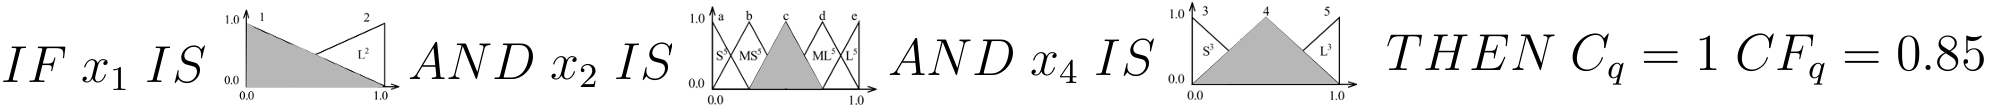
\includegraphics[width=\textwidth]{fig/fuzzy_rule.png}
                    \end{center}
                    \caption{Example rule decoded from the individual
                    chromosome (attribute $x_3$ was omitted in this rule)}
                    \label{fig:fuzzy_rule}
                \end{figure}  
        \end{itemize}
    \item Individual evaluation
        \begin{itemize}
            \item To ensure proper genetic algorithm process an appropriate
                fitness function must be defined \cite{bib10}, \cite{bib21}. 
                Firstly the nature of pattern recognition task must be taken 
                into account and secondly the structure of the fuzzy algorithm. 
                Generally, the main goal is
                to generate rules with the highest $CF_r$ grade, the smallest number
                of attributes and the highest classification rate. Fitness
                function is given by eq. (\ref{eq:fuzzy_fitness})
                \begin{equation}
                    F_{fg} = w_1\cdot NC + w_2\cdot NNC + (\frac{1}{NOF})^2 +
                    w_3\cdot CF
                    \label{eq:fuzzy_fitness}
                \end{equation}
                where $w_1$, $w_2$ are weights for a reward and punishment to
                the rule based on the classification result (in simulations
                $w_1=5$, $w_2=10$); $NC$ and $NNC$ are
                the numbers of correctly recognized and misclassified patterns
                by a particular rule, respectively; $NOF$ is the number of
                attributes used by the rule (in the above example $NOF=3$);
                $CF$ is the strength factor of the rule and $w_3$ is the
                weight (in the simulations $w_3=10$).
                The best individuals are those which maximize function $F_{fg}$
        \end{itemize}
    \item Cross-over, mutation and population generation
        \begin{itemize}
            \item From the whole population two individuals are chosen
                randomly to constitute father and mother parents. With a
                probability of $0.5$ each allele is picked either from mother
                or father chromosome. In this way two new
                individuals are generated (see example in fig. \ref{fig:cross_over})
                \begin{figure}[H]
                    \begin{center}
                        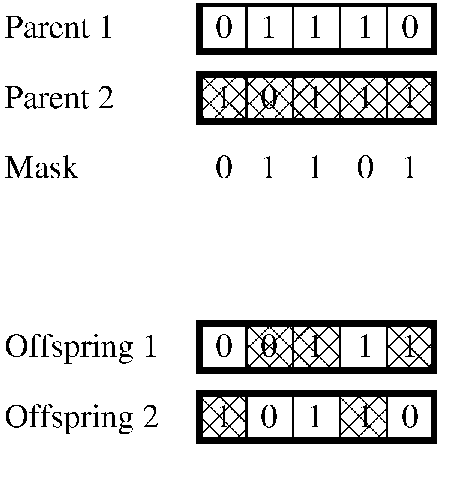
\includegraphics[width=0.6\textwidth, height=0.5\textwidth]{fig/cross_over.png}
                    \end{center}
                    \caption{Cross-over operation used in genetic algorithm}
                    \label{fig:cross_over}
                \end{figure}
            \item In the particular generation one chromosome is chosen
                randomly and later in each allele new membership function is
                taken from other possible functions. For example if in the first
                allele the first membership function is chosen the set of
                candidates is given by $\{2, \ldots, 9, a, \ldots, e, DON'T\, USE\}$
            \item In genetic algorithm one of the most important issue is how
                to generate next population \cite{bib22}. Here, after the end of one
                generation individuals from the population are merged with
                those created through cross-over and mutation operations.
                Later, the average fitness value $F_{avg}$ is calculated in the whole
                set. To the next generation those individuals are passed which
                their fitness indicator $F_{fg}$ is greater than the average
                $F_{fg} \ge F_{avg}$
        \end{itemize}
\end{itemize}
Of course it can happen that for cross-over and mutation operator
newly-generated individual will be invalid (the whole chromosome contains only
$DON'T\; USE$ linguistic variables). In such a situation rule is rejected and
the whole generation process is repeated again.

Table \ref{tab:fuzzy_genetic_parameters} presents basic genetic algorithm parameters.
Optimal values were determined during simulations by trial and error method.
\begin{table}[H]
    \caption{Parameter settings for genetic algorithm used in fuzzy logic}
    \centering
    \begin{tabular}{|c|c|}
        \hline
        Parameter & value \\ \hline \hline
        $N_{rule}$ & 10 \\ \hline
        $N_{replace}$ & $N_{rule}/2$ \\ \hline
        Crossover probability & 0.9 \\ \hline
        Mutation probability & 0.3 \\ \hline
        Generations & 500 \\ \hline
    \end{tabular}
    \label{tab:fuzzy_genetic_parameters}
\end{table}
\subsection{Multistage hybrid algorithm construction}
\label{cha:Multistage}
\subsubsection{Motivations}
\label{cha:Mutlistage_motivations}
When we deal with complex data it can happen that a single classifier is not
sufficient. There arises a question if connection of different classifier will
improve the classification? In this thesis the hybridization of rough sets and
fuzzy logic is proposed and investigated. The next subsections show algorithm construction.
\subsubsection{Rough sets and genetic algorithm}
\label{cha:Multistage_rough_genetic}
Rough sets algorithm presented in section \ref{cha:Algorithm_construction_rough_set} uses an 
arbitrary chosen step of granulation and each attribute has the same
granulation intervals. In some cases this approach gives good results in more
complex problems algorithm efficiency is low \cite{bib24}, \cite{bib29}. Additionally, the basic rough set
algorithm uses all attributes for rule construction.

Finding the optimal attribute reduct and rough set partition is $NP$ problem \cite{bib19}, \cite{bib1}.
To overcome this obstacle a genetic algorithm is used in the similar way as in section
\ref{cha:Fuzzy_logic_genetic_algorithm}. Now, a single individual describes the
partition for each attribute independently. Reconsider individual encoding for
$4$-dimensional Iris dataset. The number of granulation intervals for each attribute is
chosen from the set $\{1, 2, \ldots, K_{max}\}$, where $K_{max}$ is the maximum
value of discretization. Additionally, $DON'T\; USE$ variable is used to
determine that a given attribute is excluded from the rule. The example of
individual is given below:
$$|2|DON'T \; USE|K_{max}|3||120$$
It means that the first feature is divided into two intervals, the second is
not used and the third and fourth are discretized into $K_{max}$ and 3
intervals, respectively. The fitness indicator of this individual is $120$.
To evaluate individual the following fitness function given by eq.
(\ref{eq:rough_fitness}) is proposed:

\begin{equation}
    F_{rg} = w_1\cdot NC + w_2\cdot NNC + (\frac{1}{NOF}) +w_3\cdot (\frac{1}{NOCR})^2
    \label{eq:rough_fitness}
\end{equation}

where $w_1$, $w_2$ are weights for a reward and punishment to
the individual on the classification result ($w1=5$, $w_2=10$); $NC$ and $NNC$ are
the numbers of correctly recognized and misclassified patterns; $NOF$ is the number of
attributes used by the rule (in the example above $NOF=3$);
$NOCR$ is the number of certain rule which are derived from
partition given by the individual; $w_3$ is the weight (in the simulations
$w_3=10$).


The whole procedure of constructing genetic rough sets algorithm can be summarized in few steps:
\begin{enumerate}
    \item Determine the maximum partition value for each attribute $K_{max}$. In
        this thesis $K_{max}$ is the same for all features
    \item Generate $N_{pop}$ individuals by randomly assigning value from the
        set $\{1, 2, \ldots, K_{max}, \, DON'T\; USE\}$ to each allele in the
        chromosome
    \item Treat each individual as a rough set partition and calculate lower,
        upper approximations and the boundary region. Evaluate individual using
        fitness function $F_{rg}$
    \item Generate $N_{replace}$ individuals using genetic operators and merge
        with the current population
    \item Choose $N_{pop}$ individual for the next generation
    \item If stopping criteria is not fulfilled go to $2$
\end{enumerate}
Cross-over and mutation operations are done in the same way as presented in
section \ref{cha:Fuzzy_logic_genetic_algorithm}. Parameters for genetic algorithm 
used in this section are presented in table \ref{tab:rough_genetic_parameters}:
\begin{table}[H]
    \caption{Parameter settings for genetic algorithm used in rough sets}
    \centering
    \begin{tabular}{|c|c|}
        \hline
        Parameter & value \\ \hline \hline
        $N_{pop}$ & 10 \\ \hline
        $N_{replace}$ & $N_{pop}/2$ \\ \hline
        Crossover probability & 0.9 \\ \hline
        Mutation probability & 0.2 \\ \hline
        Generations & 100 \\ \hline
    \end{tabular}
    \label{tab:rough_genetic_parameters}
\end{table}
In case of genetic algorithm for rough set $100$ generations were sufficient to
obtain reliable results.
\subsection{Hybrid rough sets and fuzzy logic}
\label{cha:Multistage_rough_fuzzy}
Multistage classifier created in this thesis can be divided into three phases:
\begin{enumerate}
    \item Rough sets classifier construction using genetic algorithm presented
        in section \ref{cha:Multistage_rough_genetic}
    \item Fuzzy logic classifier construction with rule generation by heuristic
        approach described in \ref{cha:Fuzzy_logic_genetic_algorithm}
    \item Pattern recognition using sequential hybrid classifier 
\end{enumerate}
Each step plays an important role in the whole process and affects the final
classification accuracy \cite{bib12}, \cite{bib27}, \cite{bib32}. Proper parameters of genetic algorithm are especially
important. The whole hybrid algorithm can be summarized in the following steps:
\begin{enumerate}
    \item Divide available dataset into three separated subsets: the first for
        genetic algorithm operation, the second and third as training and
        testing.
    \item Train rough sets, fuzzy logic classifiers
    \item Classify pattern using rough sets algorithm:
        \begin{itemize}
            \item If pattern is classified by a \textit{certain} or
                \textit{possible} rule then it is a final label
            \item If no proper rule is found or more than one rule have the same
                strength, but different label then pattern is rejected and
                processed by fuzzy logic classifier.
        \end{itemize}
\end{enumerate}
An illustrative scheme of hybrid classifier is presented in fig. \ref{fig:schematic}.
\begin{figure}[H]
    \begin{center}
        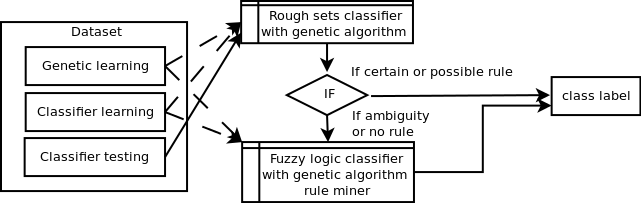
\includegraphics[width=\textwidth]{fig/diagram.png}
    \end{center}
    \caption{Schematic diagram how hybrid classifier works}
    \label{fig:schematic}
\end{figure}

\newpage\clearpage
\section{Experimentation system}
\label{cha:ExperimentAnalysis}
\subsection{Assumptions}
This section starts the second part of this thesis. In the first, algorithms
were presented in case of construction and their properties. For the simulation 
purposes the following algorithms have been implemented:
\begin{enumerate}
    \item Basic Rough sets algorithm
    \item Rough sets algorithm with modification of decision rules basing on
        the granulation step $G$
    \item Hybrid algorithm consisting of:
        \begin{itemize}
            \item Rough sets algorithm with genetic approach for finding the
                optimal partition in feature space and attribute reduction 
            \item Fuzzy logic algorithm with genetic approach for constructing
                decision rules
        \end{itemize}
\end{enumerate}

\subsection{Datasets}
\label{cha:Datasets}
To perform all the experiments, testing datasets from \textit{UCI} repository were used \cite{bib47}.
This approach is commonly used in the literature because ensures that someone
in the future would be able to retake the tests and compare the results. 
The main motivation in choosing those datasets was to ensure diversity and test
algorithms with complicated and complex problems. Below each dataset is shortly
described:
\begin{itemize}
    \item Dataset name: Haberman
        \begin{itemize} 
            \item \#attributes: 3
            \item \#instances: 306
            \item \#classes: 2
            \item Description:
                This dataset contains cases from a study that was conducted
                between 1958 and 1970 at the University of Chicago's Billings Hospital 
                on the survival of patients who had undergone surgery for breast cancer.
        \end{itemize}
    \item Dataset name: Iris
        \begin{itemize}
            \item \#attributes: 4
            \item \#instances: 150
            \item \#classes: 3
            \item Description:
                This dataset is one the most commonly used in
                pattern recognition task. Attribute information:
                \begin{itemize}
                    \item sepal length in cm 
                    \item sepal width in cm 
                    \item petal length in cm 
                    \item petal width in cm 
                \end{itemize}
        \end{itemize} 
    \item Dataset name: Wine
        \begin{itemize}
            \item \#attributes: 13
            \item \#instances: 178
            \item \#classes: 3
            \item Description:
                These data are the results of a chemical analysis of wines
                grown in the same region in Italy but derived from three 
                different cultivars. The analysis determined the quantities 
                of 13 constituents found in each of the three types of wines. 
        \end{itemize}

    \item Dataset name: Thyroid
        \begin{itemize}
            \item \#attributes: 5
            \item \#instances: 215
            \item \#classes: 3
            \item Description:
                This dataset was created at the University of
                California at Irvine by Ross Quinlan during his visit in 1987 for
                the 1987 Machine Learning Workshop. It contains 5 features
                describing thyroid symbptoms.
        \end{itemize}

    \item Dataset name: Bupa
        \begin{itemize}
            \item \#attributes: 6
            \item \#instances: 345
            \item \#classes: 2
            \item Description:
                The first 5 variables are all blood tests which are thought to
                be sensitive to liver disorders that might arise from excessive 
                alcohol consumption. Each line in the bupa.data file constitutes
                the record of a single male individual. 
        \end{itemize}

    \item Dataset name: Pima
        \begin{itemize}
            \item \#attributes: 8
            \item \#instances: 768
            \item \#classes: 2
            \item Description:
                This dataset comes from National Institute of Diabetes and Digestive and
                Kidney Diseases. The binary-valued decision indicates whether the
                patient shows signs of diabetes according to World Health Organization
                criteria. All patients are females at least 21 years old of Pima Indian heritage.
        \end{itemize}

    \item Dataset name: Wdbc
        \begin{itemize}
            \item \#attributes: 32
            \item \#instances: 569
            \item \#classes: 2
            \item Description:
                Features are computed from a digitized image of a fine needle aspirate (FNA) of a breast mass.
                Each real-valued features are computed for each cell nucleus.
        \end{itemize}
\end{itemize}
\subsection{Efficiency indicators}
\label{cha:indicators}
To evaluate effectiveness of algorithm it has to be consistent approach used in
all experiments and additionally a~priori knowledge about each dataset must
be know. By a-priori knowledge one should understand the label of class for
each pattern. Below, there are listed methods of algorithm fitness scoring:
\begin{itemize}
	\item Classification accuracy $CA$- the number of correctly classified
        patterns out of $O$ objects.
		\begin{itemize}
			\item The best value from $n$ probes 
				\begin{equation}
                    B=max\{CA_1, \ldots, CA_n\}
					\label{min1}
				\end{equation}
			\item The worst value from $n$ probes 
				\begin{equation}
                    W=min\{CA_1, \ldots, CA_n\}
					\label{min3}
				\end{equation}
			\item The average value from $n$ probes
				\begin{equation}
                    A=\frac{1}{n}\cdot\sum\limits_{i=1}^{n} (CA_i)
					\label{min2}
				\end{equation}
		\end{itemize}
	\item Error variance from $n$ simulations 
		\begin{equation}
            \sigma=\sqrt{\frac{1}{n-1}\sum\limits_{i=1}^n(AC_i-A)^2}
			\label{min4}
		\end{equation}
\end{itemize}
\subsection{Program description}
%-----------------------------------------------------------------------------------------
To perform all simulations in this project a program was written in
\textit{PYTHON}(more information can be found in \ref{Appendix}). 
It allows simulating all algorithms with chosen dataset and obtain
algorithm efficiency indicators. 

Program was tested on Linux platform with Intel Pentium Dual Core 2.4 GHz, 2GB
memory. To run the program one has to install \textit{Python} environment at
least in version 2.6. Because implemented algorithms have many setting parameters, 
they were written to the file so that easily change their value in testing procedure. 
Output results(efficiency indicators) are written to \textsc{csv} for further
processing. The most preferable environment for running this project is
Eclipse, free to download from the Internet. Each classifier is written in the
form of \textit{Python} class so that further extension would be very easy. An
example of classifiers usage is presented in appendix \ref{Appendix}.

\section{Simulation investigations}
This section presents environment setup and later the results of simulation
investigations. It is important to describe simulation setup so that in the
future someone could repeat test or maybe extend the application.
\label{cha:Simulation_investugations}
\subsection{Simulation environment}
When it comes to classification problems there is always a problem of how to
divide available dataset into training and testing sets. One of the most common
approach to ensure proper classifier evaluation is cross validation (more
information about cross validation methods can be found in). There are
different types:
\begin{itemize}
    \item \textbf{holdout cross validation}- data set is separated into two sets, called the 
        training set and the testing set. Classifier is trained using the 
        training set only. Then the classifier is asked to predict the output 
        values for the data in the testing set. The advantage of this method is 
        that it is usually preferable to the residual method and takes no longer 
        to compute. However, its evaluation can have a high variance, because
        it depends heavily on which data points end up in the training set and 
        which end up in the test set
    \item \textbf{Leave-one-out cross validation}- the classifier is trained on all the
        available data except for one point and a prediction is made for that
        point and stored to compute the average error from all points. 
    \item \textbf{K-fold cross validation}- the data set is divided into $k$ subsets, 
        and the holdout method is repeated $k$ times. Each time, one of the $k$ subsets 
        is used as the test set and the other $k-1$ subsets are merged together to form 
        a training set.
\end{itemize}
In this thesis $4$-fold cross validation was used. To ensure that presented
results are reliable each test was repeated 10 times.
\label{cha:Simulation_environment}
\subsection{Simulation results}
\label{cha:Simulation_results}
\subsubsection{Impact of granulation step on rough sets efficiency}
\label{cha:Simulation_reaearch_1}
The aim of this test was to find out how the discretization of feature space
affect the classification accuracy. At first the number of intervals for each
attribute is the same and denoted as $K_l$, where $l \in (1, \ldots, d)$.
Results of the simulation are presented in table
\ref{tab:simulation_research_1} where the notation is as follows:
\begin{itemize}
    \item $G$- granulation step
    \item $O$- total number of correctly recognized objects
    \item $C/CD$- number of patterns for which a certain decision rules were
        used/number of correctly recognized patterns using these rules 
    \item $P/PD$- number of patterns for which a possible decision rules were
        activated/number of correctly classified objects using these rules
    \item $V$ number of patterns rejected from classification. There was no
        suitable rule or more rules have the same strength but different class
        label.
    \item $C^*, P^*, V^*$ - total number of certain, possible, void decision rules 
        respectively
\end{itemize}
In the experiment, for every feature the initial step of granulation was
changed from 4 to 18 while the factor of its increasing $\gamma$  was equal 
to one.

Analyzing the results of simulation presented in table \ref{tab:simulation_research_1}
one can see that the quality of the algorithm depends on the step of
granulation $G$ and better results are obtained rather for small $G$.
It can be concluded that decreasing the step of granulation causes that the number of 
decision formulas with the strength equal to zero is growing. The level of
discretization is correlated with the number of cells in which decision was 
certain or possible because of predominance of one class. In a situation with a small 
number of fields there were areas with the same number of object from both class, but 
small number of void cells. Decreasing the step of granulation results in more fields 
where decision was certain for one class, but at the same time it was noticeable that 
the number of areas without representative is increasing.

\begin{table}[H]
    \caption{Result of simulation for finding the dependency between
    granulation step and classification accuracy}
    \centering
    \begin{tabular}{|c|c|c|c|c|c|c|c|}
        \hline
        $G$ & $O$ & $C/CD$ & $P/PD$ & $V$ & $C^*$ & $P^*$ & $V^*$ \\ \hline \hline
        4&114&0/0&125/95&28/19&3&7&54 \\ \hline
        5&114&0/0&121/97&32/17&2&4&119 \\\hline
        6&114&3/1&65/51&85/62&5&8&203 \\ \hline
        7&115&0/0&91/74&62/41&3&6&334 \\ \hline
        8&113&2/1&24/17&127/95&8&9&495 \\ \hline
        9&114&4/4&59/48&90/62&6&7&716 \\ \hline
        10&112&36/25&38/32&79/55&12&13&975 \\ \hline
        11&112&5/2&30/23&118/87&7&9&1315 \\ \hline
        12&111&49/41&9/4&95/66&19&12&1697 \\ \hline
        13&109&0/0&13/9&140/100&17&12&2168 \\ \hline
        14&112&9/6&28/24&116/82&24&14&2706 \\ \hline
        15&105&30/25&17/4&106/76&27&13&3335 \\ \hline
        16&108&2/1&20/17&131/90&22&12&4062 \\ \hline
        17&100&3/1&38/24&112/75&24&17&4872 \\ \hline
        18&101&2/1&11/8&140/92&25&13&5794 \\ \hline
    \end{tabular}
    \label{tab:simulation_research_1}
\end{table}

\subsubsection{Impact of recursive modification of granulation step on rough sets
efficiency}
\label{cha:Simulation_reaearch_2}
In the previous section (\ref{cha:Simulation_reaearch_2}) it was shown that the
granulation step strongly affect the classification accuracy.
Greater $G$ implies that we have more certain or possible rule, but on the
other hand number of patterns without rule covering is increasing. A lot of
patterns are rejected because no proper rule is found. To improve that
situation algorithm for modification of decision rules is proposed. More
details are presented in section
\ref{cha:Algorithm_construction_rough_set_modification}, but generally when an
object is rejected from classification $G$ is decreased by $\epsilon=1$ until 
proper certain for possible solution is found. The same dataset was used as in
the previous one with the same algorithm settings. Results of classification
are presented in fig. \ref{fig:Simulation_research_2} for the basic rough
sets (blue line-BRS) and algorithm with modification of decision rules (orange
line-MRS).
\begin{figure}[H]
    \begin{center}
        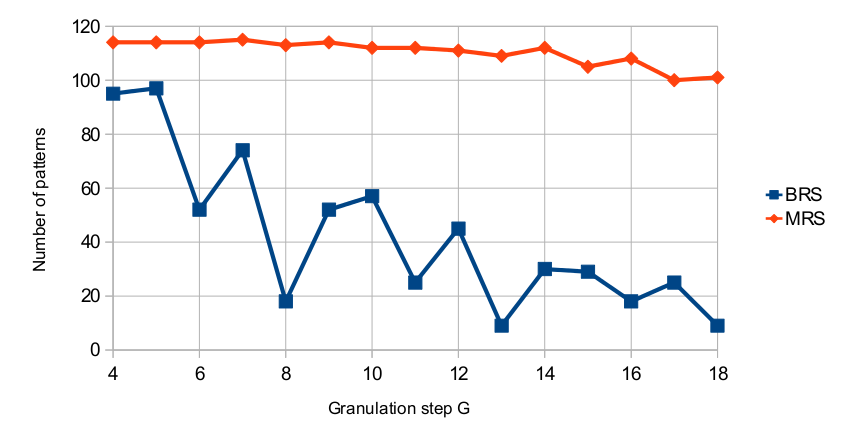
\includegraphics[width=\textwidth]{fig/rough_chart.png}
    \end{center}
    \caption{Comparison of Basic Rough sets algorithm with algorithm where
    modification of decision rules is introduced.}
    \label{fig:Simulation_research_2}
\end{figure}

Looking at fig. \ref{fig:Simulation_research_2} one can observer that
modification of granulation step $G$ increases the classification accuracy and
even if the granulation step is changed classification stays almost at the same
level while in the basic approach the greater $G$ implies worse results.
Additionally, it is visible that increasing granulation step is not the right
solution. Even if the number of certain or possible rules is greater the final
result is worse. Additionally, computational time is longer for greater $G$. In
this case the optimal $G$ would be 5, but for each problem $G$ should be chosen
independently because it must reflect how patterns are located in the feature
space.

The main two disadvantages of proposed rough sets algorithms are as follows:
\begin{itemize}
    \item it uses an arbitrary chosen step of granulation. Modification of
        decision rule improves classifier quality, but for the prize of
        computational time. 
    \item it uses all attributes for creation of decision rules. When the
        problem is complex decision rules are long and tangled. Additionally,
        some features are useless in classification, instead of valuable
        information bring noise to the system and deteriorate final results.
\end{itemize}

\subsubsection{Impact of number of membership functions on genetic fuzzy logic algorithm efficiency}
\label{cha:Simulation_reaearch_3}
In this section the results of fuzzy logic classifier simulation are presented.
The goal is to show that proposed algorithm construction is correct and gives
satisfactory results. 

At first, let remind what are the requirements for fuzzy logic classifier in
this thesis. As the input we have dataset without no expert knowledge of how to
appropriately divide feature space into fuzzy sets, how many membership
functions we need. The goal is to minimal rule set with the possible highest
classification accuracy. 

As the first step let present how fuzzy logic classifier deals with pattern
recognition and what is the minimal rule set for exemplary dataset which is
iris dataset with four attributes. At the beginning each feature was divided
into 14 membership functions in the same way as presented in fig. \ref{fig:fuzzy_example}
The final rule set which was able to classify 32 out of 34 testing pattern is
presented in fig. \ref{fig:fuzzy_result}:
\begin{figure}[H]
    \begin{center}
        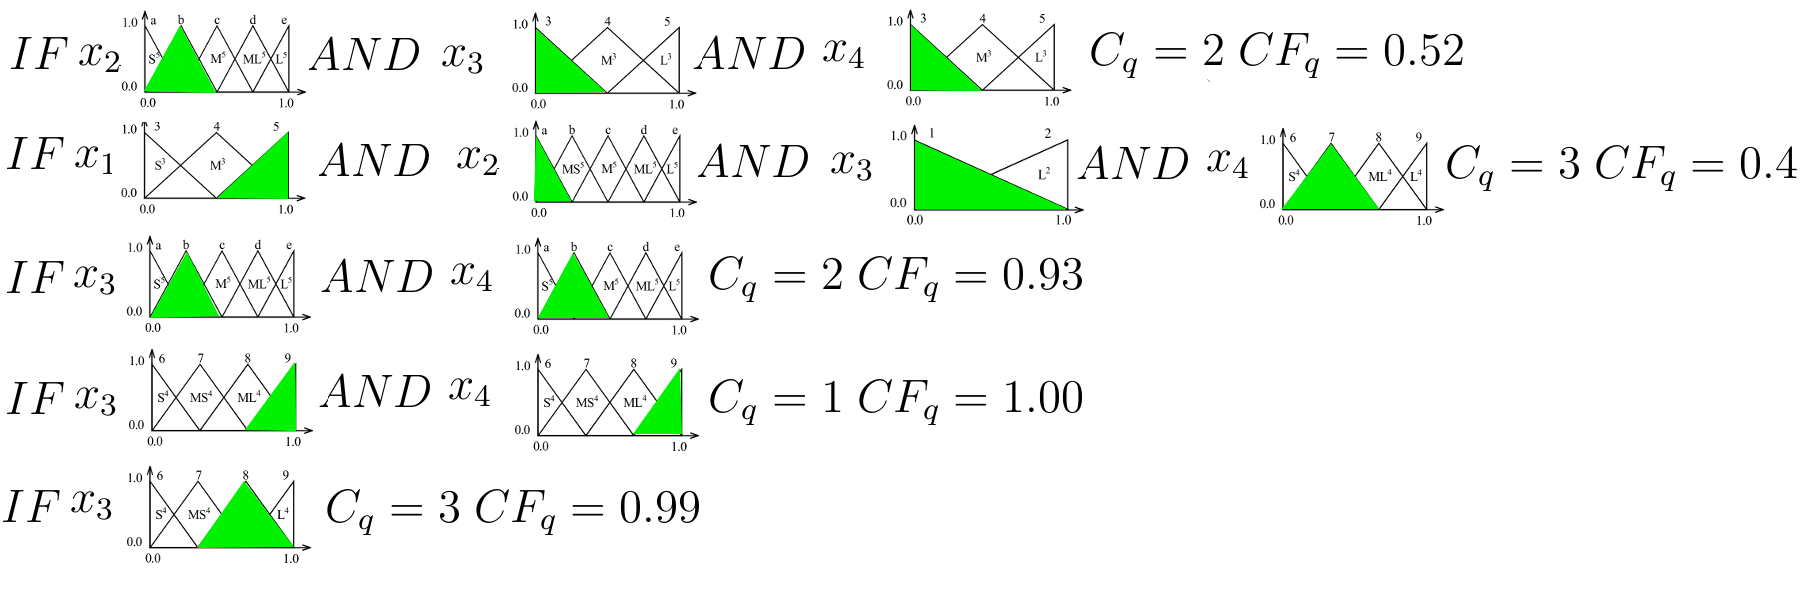
\includegraphics[width=\textwidth]{fig/fuzzy_result.png}
    \end{center}
    \caption{Example of rule set generated for Iris dataset}
    \label{fig:fuzzy_result}
\end{figure}
Analyzing figure \ref{fig:fuzzy_result} it is visible that some attributes were
omitted from classification, but the results of classification are quite
satisfactory. Additionally, only five rules were needed for correct pattern
recognition.

The goal of the second part of this test was to check how the number of initial
membership functions affects the final result of classification. There is a
question if it is better to use many small membership functions (for example 14
functions such as presented in fig. \ref{fig:fuzzy_example}}) or only few
functions with greater area coverage. In the first case the solution space is 
much greater than in the second approach so many rules must be created to obtain 
reliable results. Additionally, in most recognition problems we do not need so precise
feature partitions because it can happen that for many created regions we
cannot find proper representatives in the training set. 
Parameters for genetic algorithms are the same as presented
in table \ref{tab:fuzzy_genetic_parameters}. In each simulation the level of
partitions $k$ was changed from $7$ to $2$. Few words of explanation should be
written about how $k$ determines the number of membership functions $MF$ for each
attribute. This number is described by eq. (\ref{eq:fuzzy_function_number})
\begin{equation}
    MF = \sum\limits_1^k (n + 1) + 1
    \label{eq:fuzzy_function_number}
\end{equation}

\begin{figure}[H]
    \begin{center}
        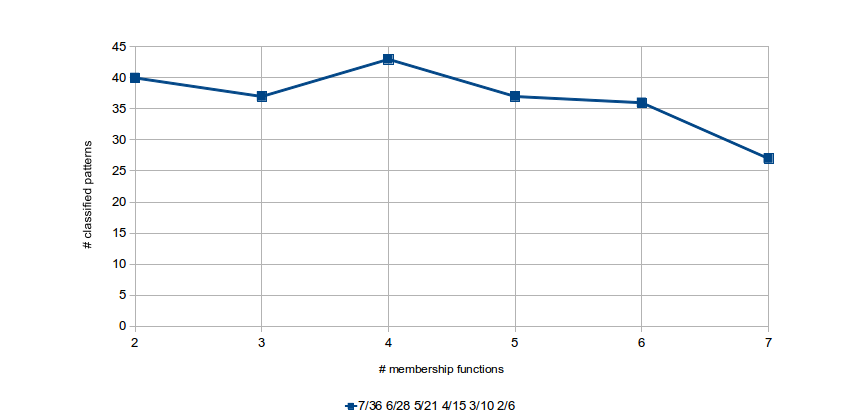
\includegraphics[width=\textwidth]{fig/fuzzy_functions.png}
    \end{center}
    \caption{Impact of initial number of membership functions $MF$ per attribute on
    the final fuzzy classification rate}
    \label{fig:fuzzy_functions}
\end{figure}
Looking at the fig. \ref{fig:fuzzy_functions} one can conclude that it is not
worth increasing the number of membership functions ($MF$) per attribute
because for greater $MF$ algorithm obtained worse results in case of
classification accuracy. From conducted simulations it was concluded that the
optimal $k$ value is 4. If not implicitly stated, $k=4$ will be used in next
tests.

\subsubsection{Impact of granulation step $G$ on genetic rough sets algorithm efficiency}
\label{cha:Simulation_reaearch_4}
The goal of this test is to check which approach is better:
\begin{enumerate}
    \item use the same granulation step $G$ for each attribute and additionally
        take all feature into classification
    \item use different partition for each attribute independently and try to
        remove some features treating them as a noise.
\end{enumerate}
The first approach is simulated by algorithm with modification of decision
rules (see section
\ref{cha:Algorithm_construction_rough_set_modification}), while the second
is genetic rough sets algorithm (described in section \ref{cha:Multistage}),
where the notation is as follows:
\begin{itemize}
    \item $A$ number of attributes describing pattern in dataset
    \item $O$ number of patterns for classification
    \item $RSR$ number of objects correctly recognized by basic rough sets
        algorithm
    \item $RSMR$ number of patterns correctly recognized by rough sets
        algorithm with modification of decision rules
    \item $GRR$ number of objects correctly recognized by genetic rough sets
        algorithm
    \item $AU$ number of features used by genetic rough sets algorithm for
        classification.
\end{itemize}

Results of simulation are presented in table \ref{tab:genetic_rough_results}.
Parameters for genetic rough sets algorithm were the same as presented in table
\ref{tab:rough_genetic_parameters} and for the first rough sets algorithm
granulation step $G$ was equal to 5 and for algorithm with modification of
decision rules starting granulation value was $7$.
\begin{table}[H]
    \centering
    \begin{tabular}{|c|c|c|c|c|c|c|}
        \hline
        Dataset & $A$ & $O$ & $RSR$ & $RSMR$ & $GRR$ & $AU$\\ 
        \hline \hline
        haberman& 3&	76&	49&	58&	61 & 2 \\ \hline
        iris&	4&	39&	32&	38&	39 & 2\\ \hline
        bupa&  	6&	86&	28&	53&	57 & 3\\ \hline 
        pima&   8&	192&	69&	126& 155 & 5 \\ \hline
        wine& 13&	45&	0&	15&	44 & 2\\ \hline
    \end{tabular}
    \caption{Accuracy of classification for genetic rough sets and basic rough
    sets algorithms for different datasets}
    \label{tab:genetic_rough_results}
\end{table}
From table \ref{tab:genetic_rough_results} one can conclude that genetic rough
sets algorithm obtains better results than other algorithms, especially it is
visible for more complex problems such as wine or pima datasets. Additionally,
let analyze the last column $AU$. It determines how many attributes are used in
genetic rough sets algorithm for classification. It is noticeable that some
features are useless and genetic rough sets algorithm is able to find
valuable attributes. Another thing to reconsider is how the complexity of the
problem affects algorithm classification accuracy. Basic rough sets algorithm
tackles quite well with simple problems, for example iris or haberman datasets,
but when the number of attributes is greater than $4$ algorithm efficiency
decreases, while genetic rough sets is not affected by this problem and can
deal with complex datasets.


\subsubsection{Comparison of hybrid classifier with other classifiers}
\label{cha:Simulation_reaearch_5}
In this section results for hybrid classifier are presented. The accuracy of
classification is compared with other classifiers trained and tested with the
same datasets. The main goal of this simulation was to check if proposed
solution can compete with other classifiers. As the source of reference
different types of classifiers were chosen to ensure the greatest diversity:
\begin{itemize}
    \item LDAC classifier (Linear Discriminant classifier)- The linear
        discriminant analysis method consists of searching, some linear
        combinations of selected variables, which provide the best separation between the
        considered classes. These different combinations are called
        discriminant functions (see example in fig. \ref{fig:ldac_example})
        \begin{figure}[H]
            \begin{center}
                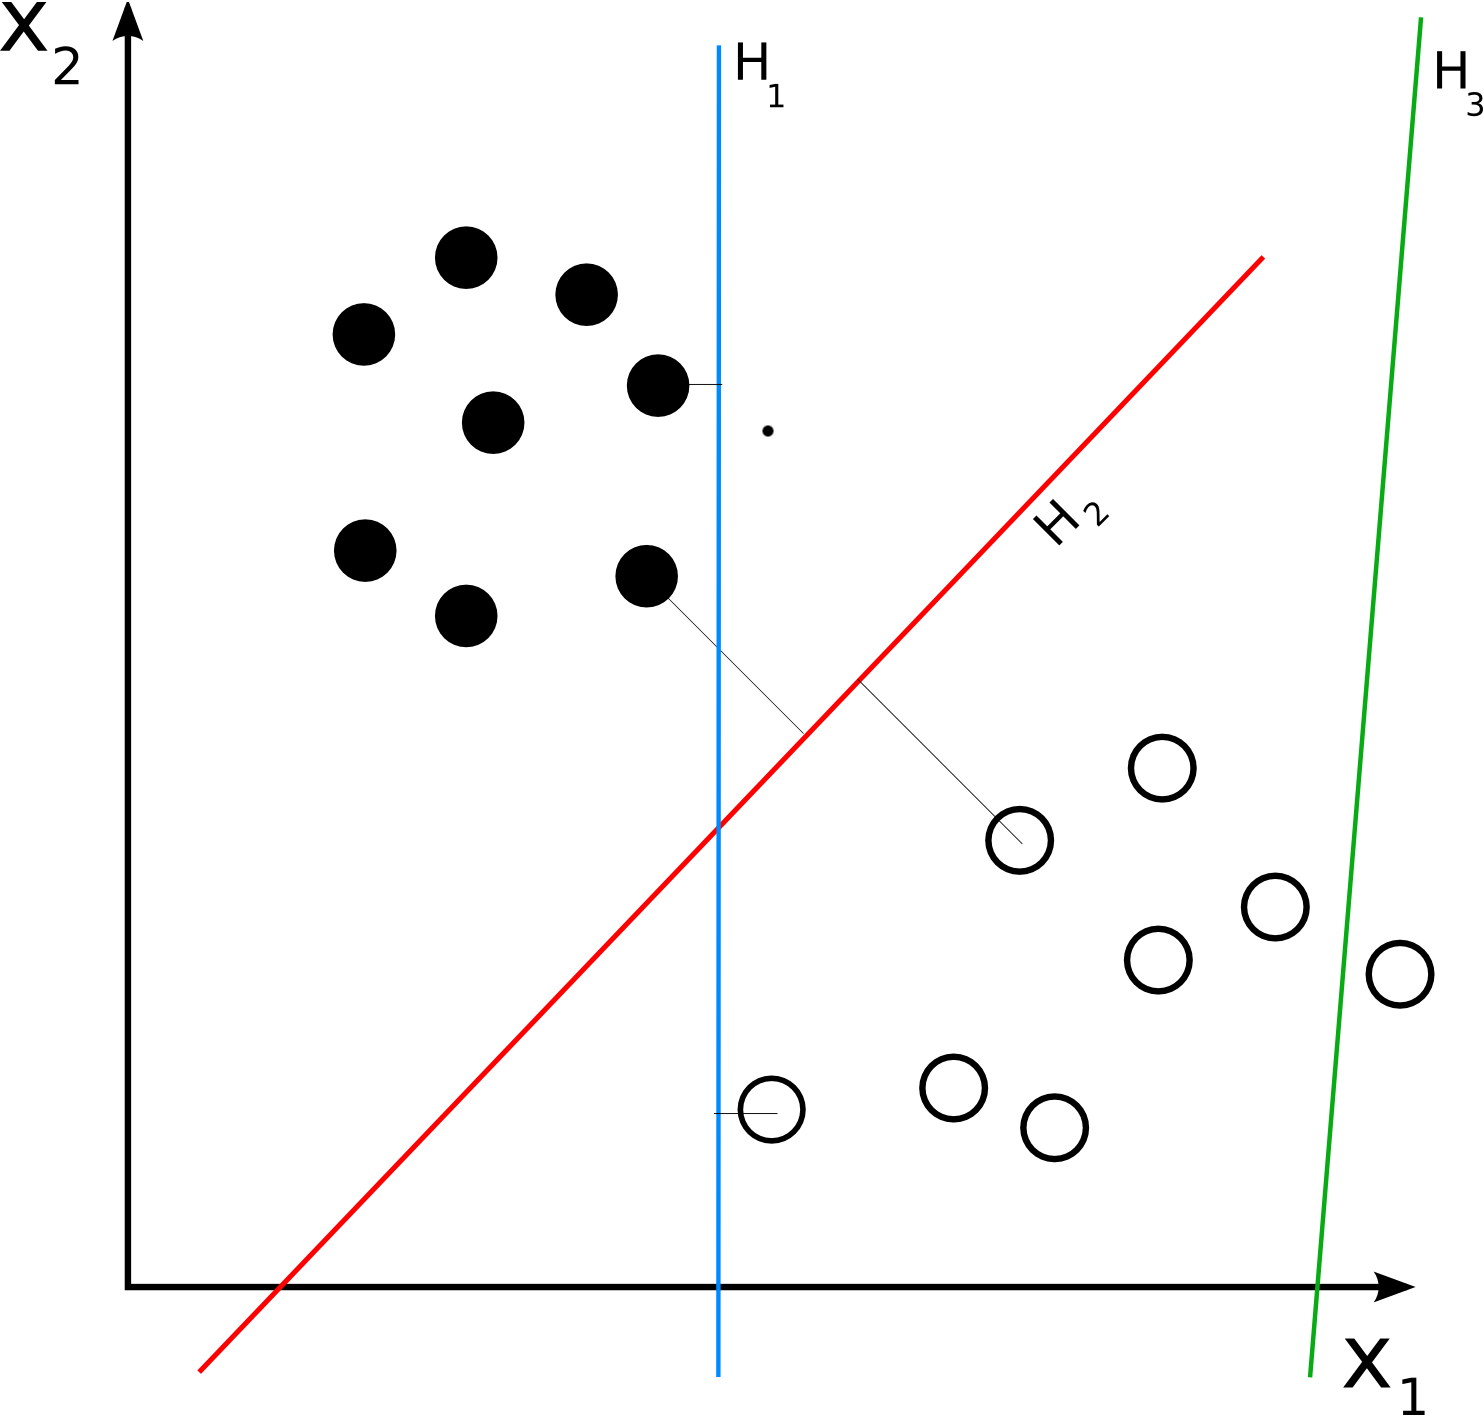
\includegraphics[width=0.6\textwidth, height=0.5\textwidth]{fig/ldac.png}
            \end{center}
            \caption{Example of linear discriminant classifier for 2-dimensional problem}
            \label{fig:ldac_example}
        \end{figure}
    \item 3-KNN Classifier- it is one of the simplest approach in the pattern
        recognition, it classifies objects based on closest training examples
        in the feature space.
    \item Gini index classifier- it is an example of decision tree algorithm
        where the decision is represented in case of decision rules.  Decision
        node specifies a test on a single attribute, leaf node indicates the
        value of the target attribute, arc/edge splits of one attribute and
        path indicated the disjunction of test to make the final decision. 
        Decision trees classify instances or examples by starting at the root 
        of the tree and moving through it until a leaf node is reached.
    \item Maximum likelihood classifier- this classifier is commonly used in
        image recognition tasks. It assigns a pixel to a class on the basis of
        its probability of belonging to a class whose mean and covariance are
        modelled as forming a normal distribution in multidimensional feature
        space.
    \item Svm classifier- it is non-probabilistic linear classifier which 
        deals with finding an optimal linear hyperplanes for class separation.
\end{itemize}
Results of simulation are presented in table \ref{tab:final_comparison}, where
$O$ determines the number of patterns for classification. Last row in table
shows results for hybrid classifier described in section
\ref{cha:Multistage_rough_fuzzy}. Numbers in bold font indicates which
classifier obtained the best result for a particular dataset.

\begin{table}[H]
    \caption{Comparison of hybrid rough fuzzy classifier with other common
    classifiers}
    \centering
    \begin{tabular}{|c|c|c|c|c|c|c|c|}
        \hline
        Algorithm&iris&bupa&pima&haberman&wine&wdbc&thyroid \\ \hline \hline
        $O$&39&86&192&76&45 & 142 & 55\\ \hline
        LDAC&38&62&146&58&44& \textbf{138} &51 \\ \hline
        3-KNN&38&56&131&56&32 & 133 &52 \\ \hline
        Gini Index&38&56&123&58&41& 131 &53 \\ \hline
        Max likelyhood&38&51&145&58&45 & 135 &55\\ \hline 
        Svm&26&\textbf{63}&141&56&43& 133 & 53\\ \hline \hline
        \textbf{Hybrid}&\textbf{39}&59&\textbf{155}&\textbf{61}&\textbf{45}&
        135 & \textbf{55}\\ \hline
    \end{tabular}
    \label{tab:final_comparison}
\end{table}

From table \ref{tab:final_comparison} one can conclude that hybrid classifier
obtains quite good results comparing with other classifiers. From seven
datasets five times it was the best. In other cases results are comparable.
What is more important hybrid classifier is able to classify pattern with
reduced number of attributes. In this case created decision rules are simpler
and more readable for user. This is especially important in medicine where
physician is provided with decision rules and basing on them makes the final
diagnosis. Another thing to reconsider is the stability of proposed classifier.
It uses genetic algorithm for rule construction, so taking into account its
random nature hybrid classifier can be unstable, but simulations show that this
is not a problem. Appropriate number of generations for genetic algorithm
assures proper convergence and as the consequence hybrid classifier is stable. 

\newpage\clearpage
\section{Summary and conclusions}
\label{cha:Summary}
\subsection{Conclusions from tests}
In this paper the results of simulation investigations were presented. The main
purpose of five test scenarios was to evaluate prepared classifiers in case of
classification accuracy. Implemented and tested algorithms in this paper are as follows:
\begin{enumerate}
    \item Basic Rough sets algorithm
    \item Rough sets algorithm with modification of decision rules
    \item Genetic Based Fuzzy Logic algorithm
    \item Multistage hybrid classifier using Rough sets and Fuzzy logic
\end{enumerate}
Author intention was to present the whole process of constructing complex
classifier from simpler ones. Researches started with the basic rough sets
algorithm. Because the results of classification were not satisfactory new
algorithm with modification of decision rules was introduced. Significant
improvement was visible for simple problems, but for multidimensional datasets
the classification accuracy remained poor. The next proposal consisted in
constructing multistage hybrid classifier where the power of fuzzy logic and
rough sets reasoning were connected. Original algorithm presented in this
thesis used genetic algorithm for finding the reduct of attributes and the
optimal granulation step $G$ for each attribute in case of rough sets and for
fuzzy logic genetic algorithm determined the best decision rule set. 
Conducted test confirmed that proposed algorithm can compete with other classifiers 
and obtains reliable results. Next paragraphs will shortly summarize each research. 

The main goal of the first simulation was to check how the granulation step $G$
affects the classification accuracy. The efficiency of rough sets algorithm is
determined by the number of \textit{certain} and \textit{possible} rules. Ideally, it would be
great that all rules are \textit{certain} and we have 100\% coverage in the rule set.
Conveyed simulations confirmed the thesis that granulation step has the
greatest impact on the classification results. This parameter must be chosen
very carefully and few factors must be taken into account:
\begin{itemize}
    \item the complexity of the problem, how many attributes are used to
        describe the pattern,
    \item how the granulation intervals are generated, equally for all
        attributes or independently,
\end{itemize}
Another important conclusion from the first test concerns the optimal value for
$G$. It is not worth increasing $G$, good results of classification are
obtained rather for small numbers such as five or six. As the evidence analyze
table \ref{tab:simulation_research_1} where for $G=18$ the classification accuracy
was very poor. Increasing $G$ ensures that the number of \textit{certain} decision rules
is greater, but on the other hand there are more dummy rules (rule with
strength equal to 0). 

Taking into account the fact that the classification accuracy of algorithm
presented in section \label{cha:Simulation_reaearch_1} was not satisfactory,
the recursive rough sets algorithm was proposed to tackle with situation where
for the particular granulation $G$ there is no appropriate rule in the rule sets. From
simulations it can be concluded that this approach improved the classification
significantly and what is more important, thanks to the modification of
decision rules algorithm was not affected by the granulation step $G$. The stability
of classifier is the biggest advantage, but on the other hand the main drawback
is connected with algorithm execution. In situation when the pattern is rejected
from classification algorithm is recursively invoked until a proper rule is
found. This requires much more time than the basic approach without rule
modification.  For simple classification tasks this is not a problem, but for
more complex datasets algorithm computation is much longer.

This thesis concerns the problem of classifying unknown patterns using rough
sets approach and fuzzy logic reasoning. To successfully accomplish this task
new algorithm of fuzzy logic had to be implemented. In the literature there are
many examples of fuzzy logic controllers or classifiers. In this paper genetic
based fuzzy logic classifier was implemented. The main advantages of proposed
solution are as follows:
\begin{itemize}
    \item it manages to construct decision rules without any expert knowledge.
        It means that the input to the system constitutes only raw data from
        dataset without additional information about the number of membership
        functions or their location in the feature space. As the output we
        obtain rule set with the highest classification rate,
    \item it is able to apply attribute reduction,
\end{itemize}
In section \label{cha:Simulation_reaearch_3} it was shown that proposed fuzzy
classifier was able to classify 32 out of 34 testing patterns from iris dataset
with  five rules (presented in fig. \ref{fig:fuzzy_result}).

As fuzzy logic was finished and genetic algorithm turned out to be a good
solution it was decided to connect genetic algorithm with rough sets and check
how this fusion works. The main goal of the heuristic approach was to find an
optimal granulation for each feature independently and try to remove those
attributes that are useless in classification. Conducted tests proved that
this direction of researches is good and gives promising results. Especially it
was visible for high dimensional datasets where the classification rate for
basic rough sets and rough sets with modification of decision rules was very
low. 

The last part in this master thesis consisted in constructing a multistage 
hybrid classifier connecting implemented by the author genetic rough sets
algorithm and genetic based fuzzy logic algorithm. There are many types and
methods of classifier fusion, but in this paper two-phased sequential
classification was proposed. Comparison with different well-known classifiers
gave optimistic results, but of course more profound test are required to fully
prove its usefulness.
\subsection{General conclusions} 
To sum up, this paper presents the result of work in the field of pattern
recognition and classification. It reviewed some of the most representative 
publications connected with rough sets, fuzzy logic and genetic algorithms.
Here an original construction of hybrid classifier has been presented. Attached
results are very promising and encourage for further more complex
investigations. Generally, pattern recognition is not an easy task and many
factors and parameters must be taken into account. Until now, no-one has
managed to invent the classifier with 100\% accuracy. Even if for one dataset
results are satisfactory, but for others classification will be worse.

\newpage\clearpage
\section{Future work}
\label{cha:FutureWork}
In this thesis the basic parameters and settings were checked for rough sets
algorithm and fuzzy logic algorithm. In the future, it is strongly recommended 
to carry out more profound simulations to fully understand behaviour of
algorithm in different environment and settings. In this thesis to evaluate
classifiers well-known datasets from \textit{UCI} Repository. This offers
reliable environment for testing, but the next step in the future work is to
apply proposed algorithm into real life problem, such as optimal control or
image pattern recognition. Using rough sets properties it would be advisable to
detect tumor tissue on CT or MRI images or bone structures for further 3D
reconstruction.

Another thing to reconsider in the next researches is how to generate partition
of feature. Here, genetic algorithm was used to find the reduct of attributes
and the number of intervals for each attribute independently. Results of
simulations confirmed the usefulness of this approach, but here arises the
question if there is another solution for finding an optimal feature
granulation. Two possible future tests:
\begin{enumerate}
    \item Testing the classification accuracy of rough sets algorithm when
        granulation is based on the frequency of patterns in the training
        dataset. This approach assumes that for clusters with many patterns the
        granulation will be more precise while in other places it would be
        sparse.
    \item Testing the classification accuracy of rough sets algorithm when
        granulation is determined by fuzzy logic and triangular membership
        functions. A concept of fuzzy discretization of feature space for a
        rough sets theoretic classifier is presented in \cite{bib100}
\end{enumerate}

The last, but not least aspect of the future work is to check different types
of classifier hybridization. In this thesis rough sets algorithm was the most
important and only in cases when pattern was rejected fuzzy logic classifier
was used. It would be required to simulate different scenarios of classifier
ensemble, for example majority voting with fuzzy logic, rough sets and neural
network or 3-KNN classifiers. Additionally, it would be great to compare
different algorithms for feature reduction with genetic approach used in this
paper. 




\newpage \clearpage
\addcontentsline{toc}{section}{Literature}
\addcontentsline{toc}{section}{List of figures}
\addcontentsline{toc}{section}{List of tables}


\begin{thebibliography}{99}

\bibitem{bib1}
Roy A., Pal K. S., : \textit{``Fuzzy discretization of feature space for rough
set classifier''}, Elsevier, Pattern Recognition Letters 24, 2004

\bibitem{bib2}
Krupka I., JIRAVA P., : \textit{``Modelling of Rough-Fuzzy Classifier''}, WSEAS
TRANSACTIONS on SYSTEMS, Issue 3, Volume 7, March 2008

\bibitem{bib3}
Khoo L.P., Zhai L., : \textit{``A prototype genetic algorithm-enhanced rough
set-based rule induction system''}, Elsevier, Computers in Industry 46, 95-106,
2001

\bibitem{bib4}
Meng D., Pei Z. , : \textit{``Extracting linguistic rules from data sets using fuzzy logic and
genetic algorithms''}, Elsevier, Neurocomputing 78, 48-54, 2012

\bibitem{bib5}
Kothari A., Keskar A., : \textit{``Feature Space Reductions Using Rough Sets for a Rough-Neuro Hybrid Approach Based Pattern
Classifier''}, Proceedings of the World Congress on Engineering and Computer Science 2008 WCECS 2008, October 22 - 24, 2008, 
San Francisco, USA

\bibitem{bib6}
Hu Q., Shuang A., : \textit{``Robust fuzzy rough classifiers''}, Elsevier, Fuzzy Sets and Systems 183, 26–43, 2011

\bibitem{bib7}
Wu W., Peirong L., : \textit{``Topological Spaces for Fuzzy Rough Sets Determined by Fuzzy Implication
Operators''}, Sixth International Conference on Fuzzy Systems and Knowledge Discovery, 2009

\bibitem{bib8}
Affanso C., Sassi R. J., : \textit{``Traffic Flow Breakdown Prediction using Feature
Reduction through Rough-Neuro Fuzzy Networks''}, Proceedings of International Joint Conference on Neural Networks, 
San Jose, California, USA, July 31 – August 5, 2011

\bibitem{bib9}
Qinghua H., Congxin W., : \textit{``Fuzzy preference relation rough sets''},
Harbin Institute a/Technology, Harbin 150001, P. R. China, 2007

\bibitem{bib6}
	Xia S. , Jamshidi M., : \textit{``A Genetic Algorithms - Discrete Event Simulation
  Methodology for Modeling and Simulation of Autonomous Systems''},
 Department of Electrical and Computer Engineering and Autonomous Control Engineering
 (ACE) Center, University of New Mexico, Albuquerque, NM 87131, 1999

\bibitem{bib12}
	Nazan K., : \textit{``Population Sizing in Genetic and Evolutionary Algorithms''},
	 Illinois Genetic Algorithms Laboratory Department of~General Engineering University 
	 of~Illinois at~Urbana-Champaign, 2003

\bibitem{bib17}
	Harik G., Cantu-Paz E., Goldberg D. E, Miller B. L., : \textit{``The Gambler’s Ruin Problem, Genetic Algorithms, and the Sizing of Populations''}, 
	Illinois Genetic Algorithms Laboratory University of Illinois Urbana, IL
	61801 USA, 1999

\bibitem{bib18}
	Chen J., : \textit{``Theoretical Analysis of Multi-Objective Genetic
Algorithms - Convergence Time, Population Sizing, and Disequilibrium''}, 
Department of Information Engineering and Computer Science Feng Chia University,
Taichung, Taiwan 407, ROC, 2000

\end{thebibliography}
\newpage
\listoffigures
\listoftables


\newpage\clearpage
\appendix
\appendix
\makeatletter
\def\Pref@section{Appendix~}
\def\@seccntformat#1{\csname Pref@#1\endcsname \csname the#1\endcsname\quad}
\makeatother

\section{Program description}
\label{Appendix}
\subsection{Installation requirements}
For the test purposes the simulator in \textit{Python} language was written. To
successfully ran this program few requirements must be met. In this master
thesis this software was executed on Linux platform and here this approach will
be described. Of course it is possible to run the program on Windows, but
proper preparation must be undertaken. Requirement for the software:
\begin{itemize}
    \item \textit{Python} in version at least 2.6
    \item NumPy
    \item SciPy
    \item mlpy library with Gsl. Steps for the proper installation:
        \begin{enumerate}
            \item sudo apt-get install python2.6-dev
            \item go to: \textit{http://www.gnu.org/prep/ftp.html}
            \item click on an ftp link close to your location
            \item find the gsl/ directory and click on it
            \item find the gsl-VERSION.tar.gz file, where version is 1.14 or greater. Click on that file to download it.
            \item In a terminal window extract the tar.gz file using tar -xzf gsl-VERSION.tar.gz and then cd to the ./gsl-VERSION 
                directory
            \item Look at the INSTALL file. It will probably tell you to run ./configure, then make, and then make install
            \item download mlpy from \textit{http://sourceforge.net/projects/mlpy/files/}
            \item unzip file and inside directory run from command line python setup.py install
        \end{enumerate}
\end{itemize}

The whole project is divided into modules and each classifier is implemented as
python class:
\begin{itemize}
    \item BasicClassifiers- this class implements basic classifiers such as:
        LDAC, 3-KNN, MaximumLikelyHood Classifier, Gini Index Classifier, svm
        Classifier
    \item RoughSetsClassifier- this class implements basic rough sets
        classifier. Depending on the chosen module it is an algorithm with
        modification of decision rules or not.
    \item GeneticFuzzyLogicClassifier- this class simulate genetic fuzzy logic
        classifier. In the beginning genetic algorithm is run to obtain the
        best decision rule set and later classification is done
    \item GeneticRoughSetsClassifier- this class implements genetic rough sets
        classifier. It comprises of two parts:
        \begin{itemize}
            \item genetic algorithm for obtaining an optimal partition for each
                feature
            \item classification procedure which uses partition from the
                previous step for pattern recognition
        \end{itemize}
    \item HybridClassifier- this class implements hybrid classifier. This is a
        multistage classifier in which rough sets algorithm is treated as the
        first classifier and fuzzy logic as the second.
\end{itemize}
\subsection{Example usage}
To run each classifier few basic steps must be done. First of all proper
parameters with cross-validation and dataset type must be chosen. Below, a
simple example is presented showing how to run genetic rough sets classifier
fir iris dataset
\lstinputlisting[language=Python]{code/example.py}


\end{document}
